\documentclass[a4paper, 14pt]{extarticle}

\usepackage{../latexDependencies/misc/preamble2}

\geometry{a4paper}

% Название дисциплины
\newcommand{\subject}{Численные методы} 

% Тип работы
% lab - для лабораторной работы 
% hw  - для домашней     работы
\newcommand{\task}{hw} 

% Номер работы
\newcommand{\taskNumber}{2-1} 

% Название работы
\newcommand{\taskNameOne}{Интерполяция Лагранжа.} 
\newcommand{\taskNameTwo}{Вычисление интерполяционного полинома} 
\newcommand{\taskNameThree}{Лагранжа.} 

% Имя студента
\newcommand{\studentName}{Очкин Н.В.}

% Имя преподававателя
\newcommand{\teacherName}{Кутыркин В.А.}

% Группа
\newcommand{\group}{ФН11-52Б}

% Вариант
\newcommand{\variant}{9}

\begin{document}

\graphicspath{ {../latexDependencies/images} } 
\normalsize

\newcommand{\printTask}{%
    \ifthenelse{\equal{\task}{lab}}{%
        лабораторной%
    }{%
        \ifthenelse{\equal{\task}{hw}}{%
            домашней%
        }{%
            Неизвестный тип задания%
        }%
    }%
}

\begin{titlepage}

    \begin{center}
        {\footnotesize \itshape Федеральное государственное бюджетное 
                       образовательное учреждение высшего образования}
    \end{center}

    \begin{minipage}[c]{0.1\textwidth}
        
\includegraphics[width=1.1\textwidth]{iconBMSTU}
    \end{minipage}
    \hfill
    \begin{minipage}[c]{0.9\textwidth}
        \centering
        \itshape
        \bfseries
        \small
        \guillemotleft Московский государственный технический университет \\
        имени Н.Э. Баумана\guillemotright \\
        (национальный исследовательский университет) \\
        (МГТУ им. Н.Э. Баумана) 
    \end{minipage}

    \vspace{0.5cm}
    \noindent\rule{\textwidth}{2pt} \\

    \noindent\uline{\textbf{ФАКУЛЬТЕТ} ФУНДАМЕНТАЛЬНЫЕ НАУКИ} \\
    \vspace{-5pt} \\
    \noindent\uline{\textbf{КАФЕДРА} ВЫЧИСЛИТЕЛЬНАЯ МАТЕМАТИКА И МАТЕМАТИЧЕСКАЯ} \\
    \vspace{-5pt} \\
    \noindent\uline{ФИЗИКА (ФН11)} \\
    \vspace{-5pt} \\
    \noindent\uline{\textbf{НАПРАВЛЕНИЕ ПОДГОТОВКИ} МАТЕМАТИКА И КОМПЬЮТЕРНЫЕ} \\
    \vspace{-5pt} \\
    \noindent\uline{НАУКИ (02.03.01)} \\

    \begin{center}
        \bfseries
        \textsc{О т ч е т} \\[10pt]
        по \printTask {} работе \textnumero {} \taskNumber
    \end{center}

    \vspace{10pt}

    \hspace{10pt} 
    \noindent \textbf{Название \printTask {} работы:} \par
    \vspace{5pt}
    \hspace{10pt} 
    \noindent \textbf{\uline{\taskNameOne}} \vspace{5pt} \\
    \null\hspace{31pt} 
    \textbf{\uline{\taskNameTwo}} \vspace{5pt} \\
    \null\hspace{31pt} 
    \textbf{\uline{\taskNameThree}}

    \vspace{10pt}

    \begin{center}
        \bfseries
        Вариант \textnumero {} \variant
    \end{center}

    \vspace{20pt}

    \hspace{10pt} 
    \noindent \textbf{Дисциплина:} \par
    \vspace{10pt}
    \hspace{10pt} 
    \noindent {\large \subject}

    \vspace{10pt}

    \begin{flushright}
        \renewcommand{\arraystretch}{3}
        \begin{tabular}{r r r}
            \multicolumn{1}{l}{Студент группы \uline{\group}} & 
            $\quad \underset{\text{(Подпись, дата)}}{\underline{\hspace{3cm}}} \quad$ & 
            \multicolumn{1}{c}{$\underset{\text{(И.О. Фамилия)}}{\uline{\textbf{\studentName}}}$} \\

            \multicolumn{1}{l}{Преподаватель} & 
            $\quad \underset{\text{(Подпись, дата)}}{\underline{\hspace{3cm}}} \quad$ & 
            \multicolumn{1}{c}{$\underset{\text{(И.О. Фамилия)}}{\uline{\textbf{\teacherName}}}$} \\
        \end{tabular}
    \end{flushright}

    \vfill

    \begin{center}
        \small
        Москва, 2024
    \end{center}
\end{titlepage}


\newgeometry{left=25mm, right=25mm, top=20mm, bottom=20mm}

\graphicspath{ {../latexDependencies/images/HW2-1} }

% Customize section, subsection, subsubsection and paragraph styles
\titleformat{\section}
  {\normalfont\large\bfseries}{\thesection}{1em}{}

\titleformat{\subsection}
  {\normalfont\normalsize\bfseries}{\thesubsection}{1em}{}

\titleformat{\subsubsection}
  {\normalfont\small\bfseries}{\thesubsubsection}{1em}{}

\titleformat{\paragraph}
  {\small\small\bfseries}{\theparagraph}{1em}{}

% \thispagestyle{empty}

% \null\newpage

% \setcounter{tocdepth}{5}
% \setcounter{secnumdepth}{5}

% \pagenumbering{roman}

% \tableofcontents
% \newpage

% \pagenumbering{arabic}
% \setcounter{page}{1}

\setstretch{1}
\linespread{1.1}

\setlength{\parindent}{0pt}

\fontsize{12pt}{16pt}\selectfont

% \definecolor{myblue}{HTML}{0A88C2}
% \definecolor{myred}{HTML}{FF1B1C}
% \definecolor{mygreen}{HTML}{386641}

% \lstdefinestyle{mystyle}{
%     basicstyle=\ttfamily\footnotesize,
%     keywordstyle=\color{myblue},
%     stringstyle=\color{myred},
%     commentstyle=\color{green!50!black},
%     showstringspaces=false,
%     frame=leftline, 
%     framesep=10pt, 
% }

% % Set the style for Python code
% \lstset{style=mystyle, extendedchars=\true}

% --------------------------------------START--------------------------------------

\section*{Задание}\vspace{-20pt}\rule{\linewidth}{0.1mm}

Для гладкой на отрезке [0;2] функции
\begin{equation*}
  f(\tau) = \cfrac{20 + 0.2 \cdot N}{1 + (20 + 0.2 \cdot N) \cdot (1 + 0.05 \cdot (54 - n)) \cdot (\tau - 1)^2} \text{,}
\end{equation*}
используя равномерную сетку с 11-ю узлами, вычислить интерполяционный полином
Лагранжа. Используя равномерную сетку с 21 узлом, представить графики функции $f$ и
вычисленного (с 11-ю равномерными узлами) интерполяционного полинома Лагранжа.
Прокомментировать результаты интерполяции.\\

Для гладкой на отрезке [0;2] функции $f$, используя чебышевскую сетку с 11-ю
узлами, вычислить интерполяционный полином Лагранжа. Используя равномерную сетку
с 21 узлом, представить графики функции f и вычисленного (с 11-ю чебышевскими
узлами) интерполяционного полинома Лагранжа.\\

Прокомментировать результаты интерполяций с равномерными и чебышевскими
узлами.

\section*{Исходные данные}\vspace{-20pt}\rule{\linewidth}{0.1mm}

\begin{gather*}
  N = 9 \qquad n = 52 \\[1em]
  f(\tau) = \cfrac{20 + 0.2 \cdot 9}{1 + (20 + 0.2 \cdot 9) \cdot (1 + 0.05 \cdot (54 - 52)) \cdot (\tau - 1)^2}
\end{gather*}

\begin{center}
  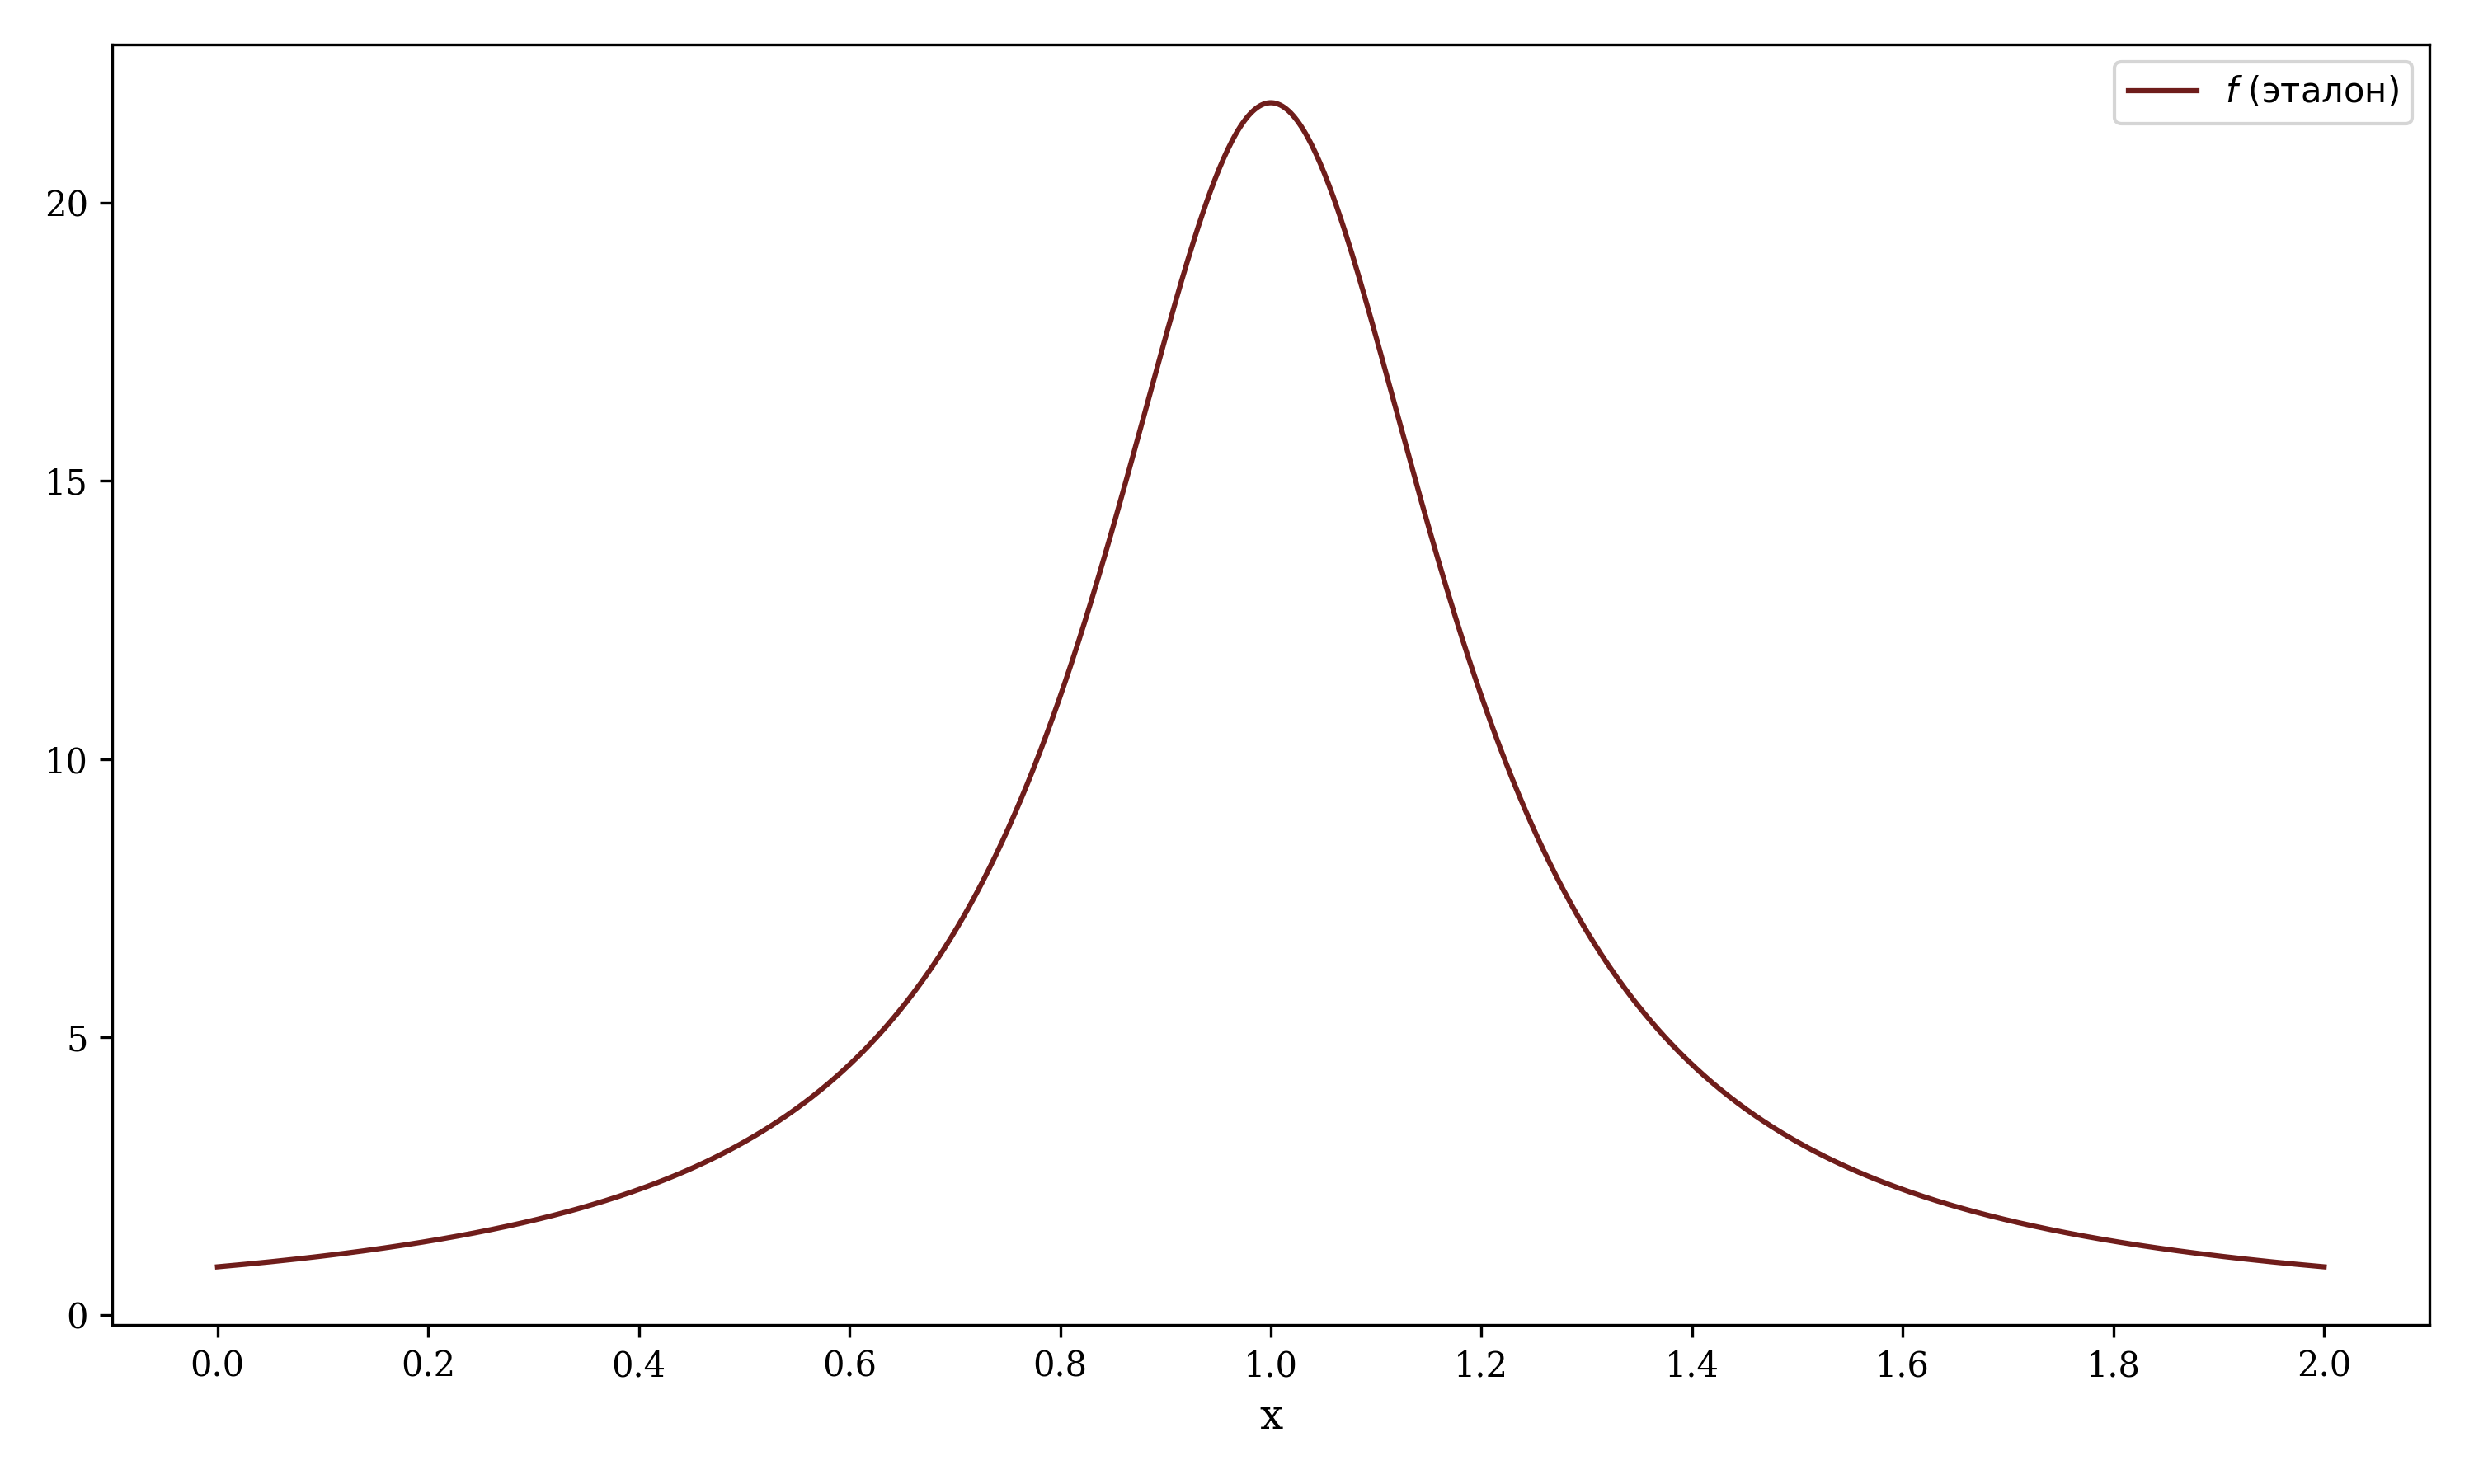
\includegraphics[width=0.8\textwidth]{ref}
\end{center}

\subsection*{Часть 1}\vspace{-20pt}\rule{\linewidth}{0.1mm}

Используя равномерную сетку с 11-ю узлами, вычислить интерполяционный полином
Лагранжа.

\paragraph*{Равномерная сетка}\vspace{-20pt}\rule{\linewidth}{0.1mm}

Для построения равнмоерной сетки с 11-ю узлами воспользуемся следующей формулой:
\begin{equation*}
  x_i = a + i \cdot h, \qquad i=0,1,2,...,10,
\end{equation*}
где $h = \frac{b - a}{10}$.\\

Также вычислим значения функции $f(\tau)$ в узлах:
\begin{equation*}
  y_i = f(x_i), \qquad i=0,1,2,...,10,
\end{equation*}

Итого получим следующие точки:
\begin{multicols}{3}
  \begin{enumerate}[itemsep=5pt]
  \item (x: 0.0, y: 0.873)
  \item (x: 0.2, y: 1.334)
  \item (x: 0.4, y: 2.263)
  \item (x: 0.6, y: 4.507)
  \item (x: 0.8, y: 11.127)
  \item (x: 1.0, y: 21.8)
  \item (x: 1.2, y: 11.127)
  \item (x: 1.4, y: 4.507)
  \item (x: 1.6, y: 2.263)
  \item (x: 1.8, y: 1.334)
  \item (x: 2.0, y: 0.873)
  \end{enumerate} 
\end{multicols}

\vfill

\begin{center}
  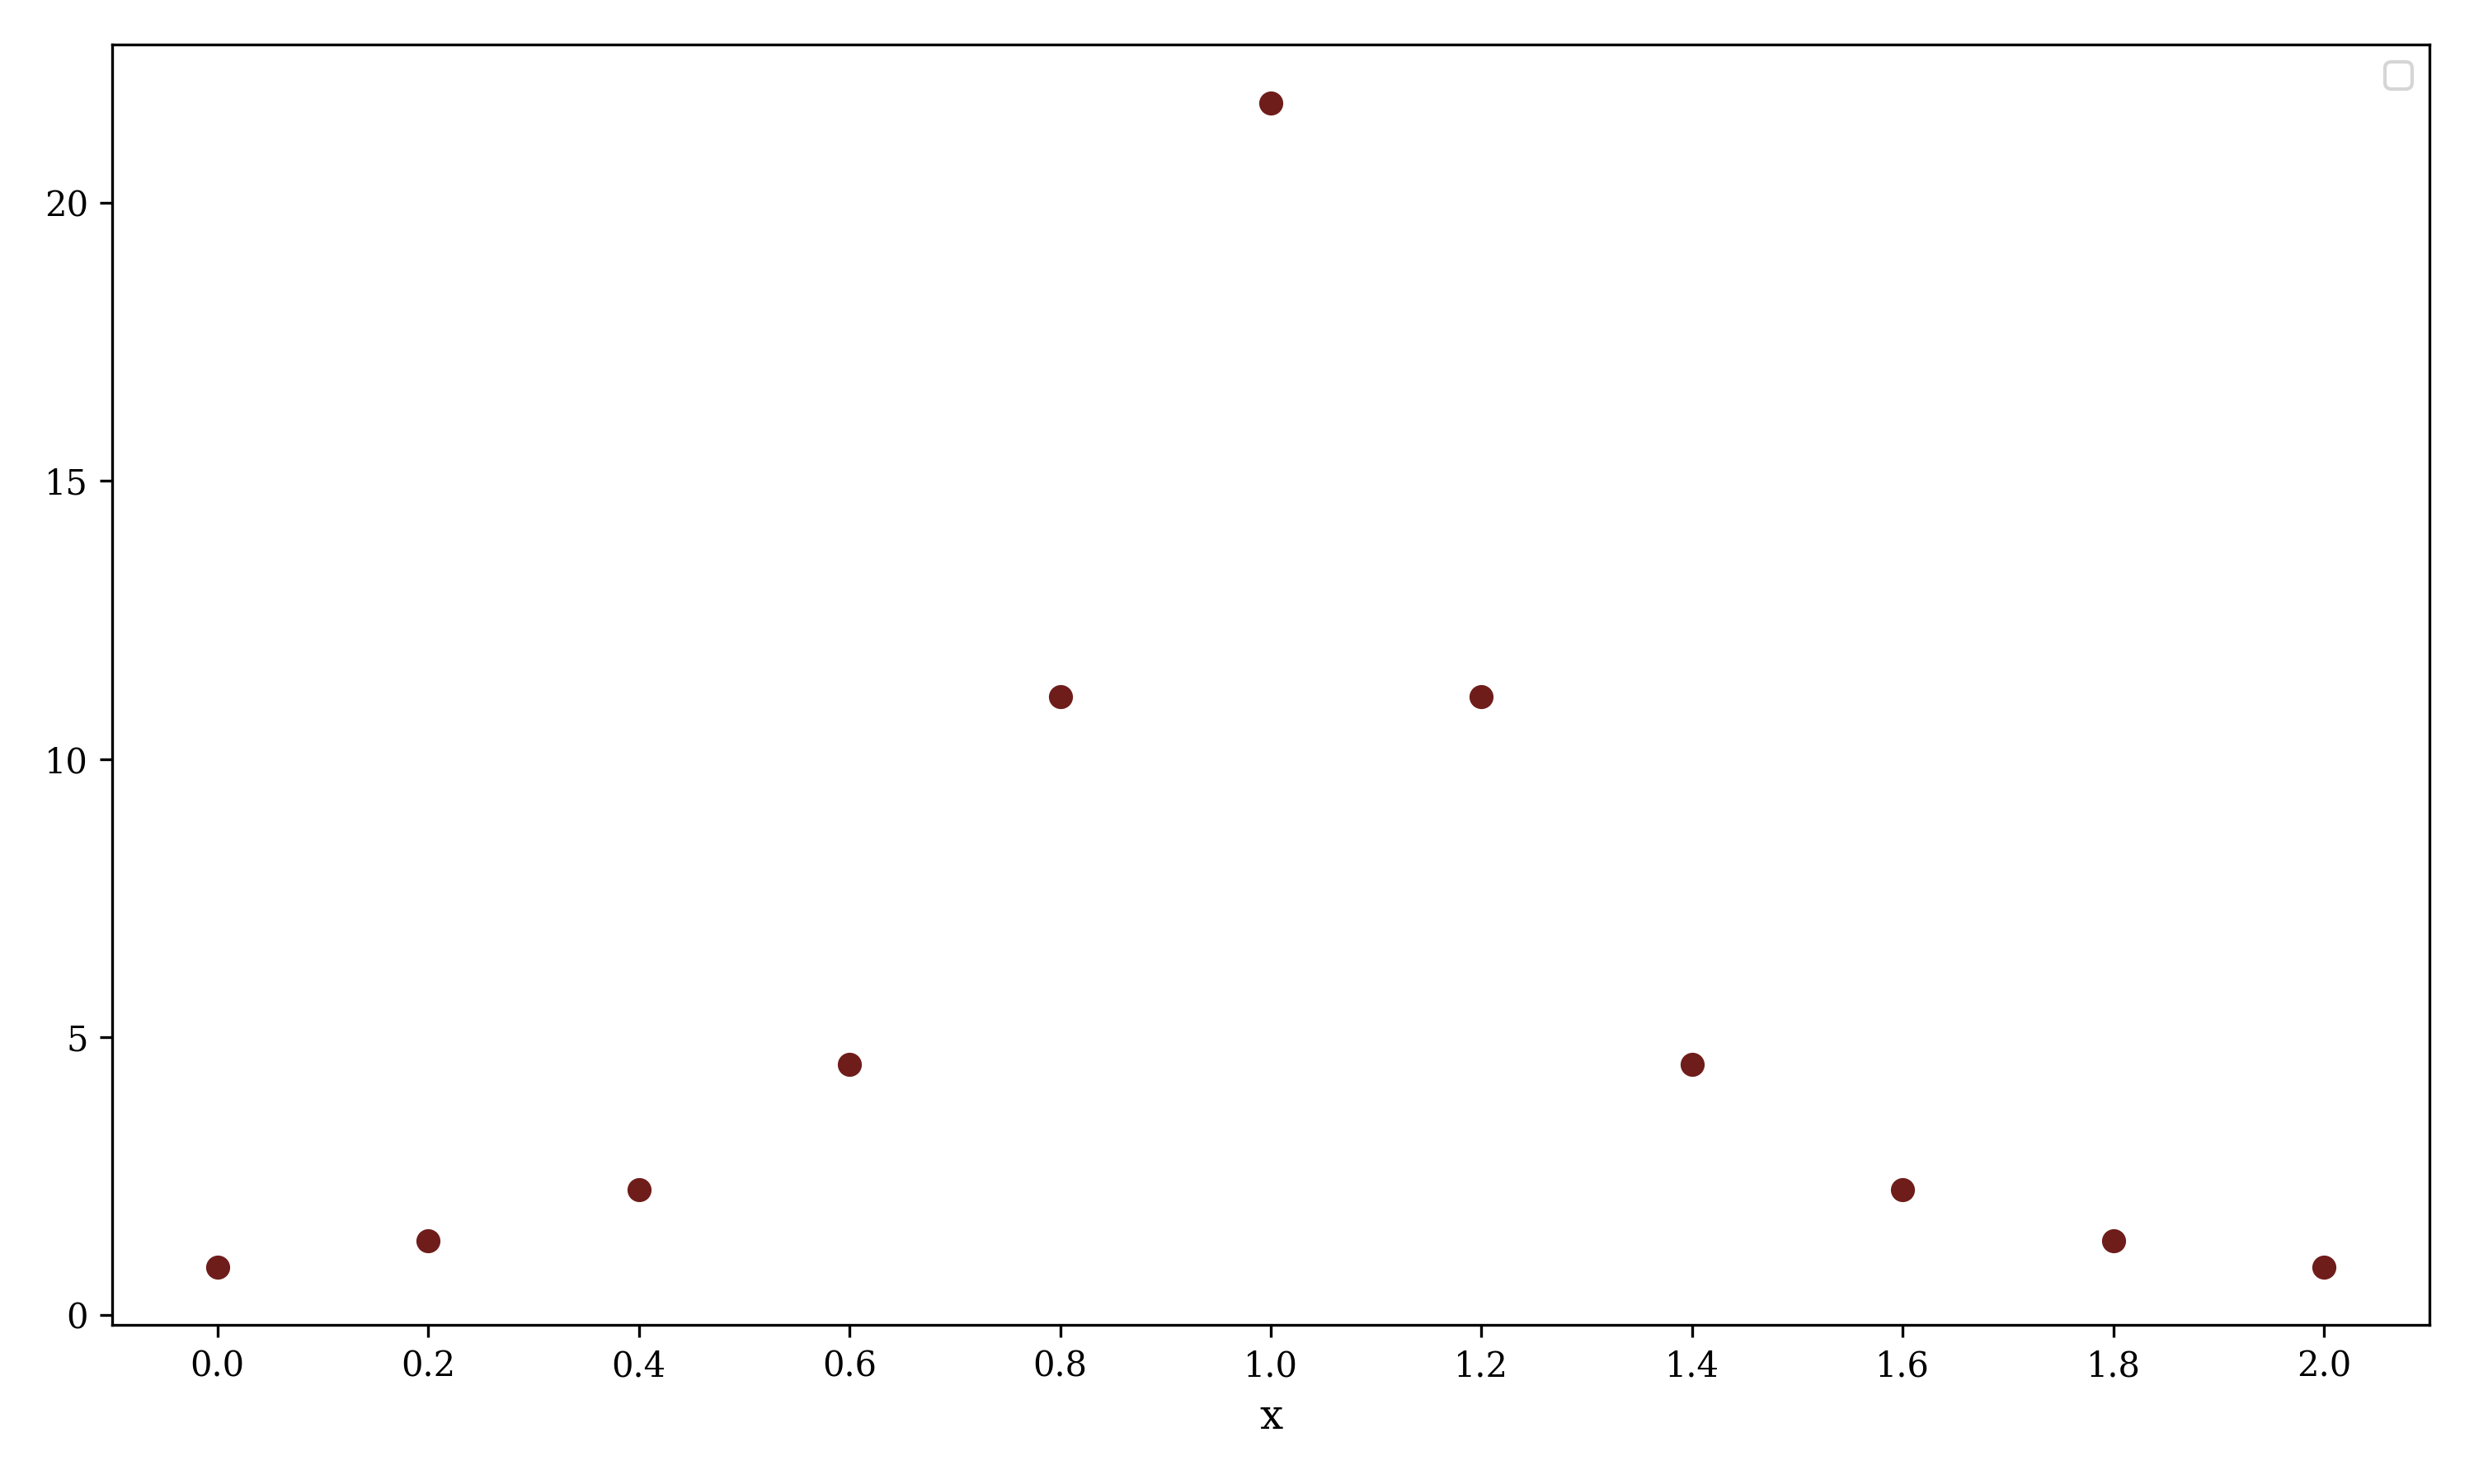
\includegraphics[width=1\textwidth]{scatter1}
\end{center}

\vfill

\newpage

\paragraph*{Интерполяционный многочлен Лагранжа (с использованием равномерной сетки с 11-ю узлами)}\vspace{-20pt}\rule{\linewidth}{0.1mm}

Интерполяционный многочлен Лагранжа будем искать по следующей формуле:
\begin{equation*}
  L(x) = \sum_{i = 0}^{n} y_i l_i(x),
\end{equation*}
где базисные полиномы $l_i$ определяются по формуле 

\begin{equation*}
  l_i(x) = \prod_{j=0, j\neq i}^{n} \cfrac{x - x_j}{x_i - x_j}
\end{equation*}

Используя равномерную сетку с 21 узлом, представим совмещенные графики функции $f$, и 
вычисленного (с 11-ю равномерными узлами) интерполяционного полинома Лагранжа.

\begin{center}
  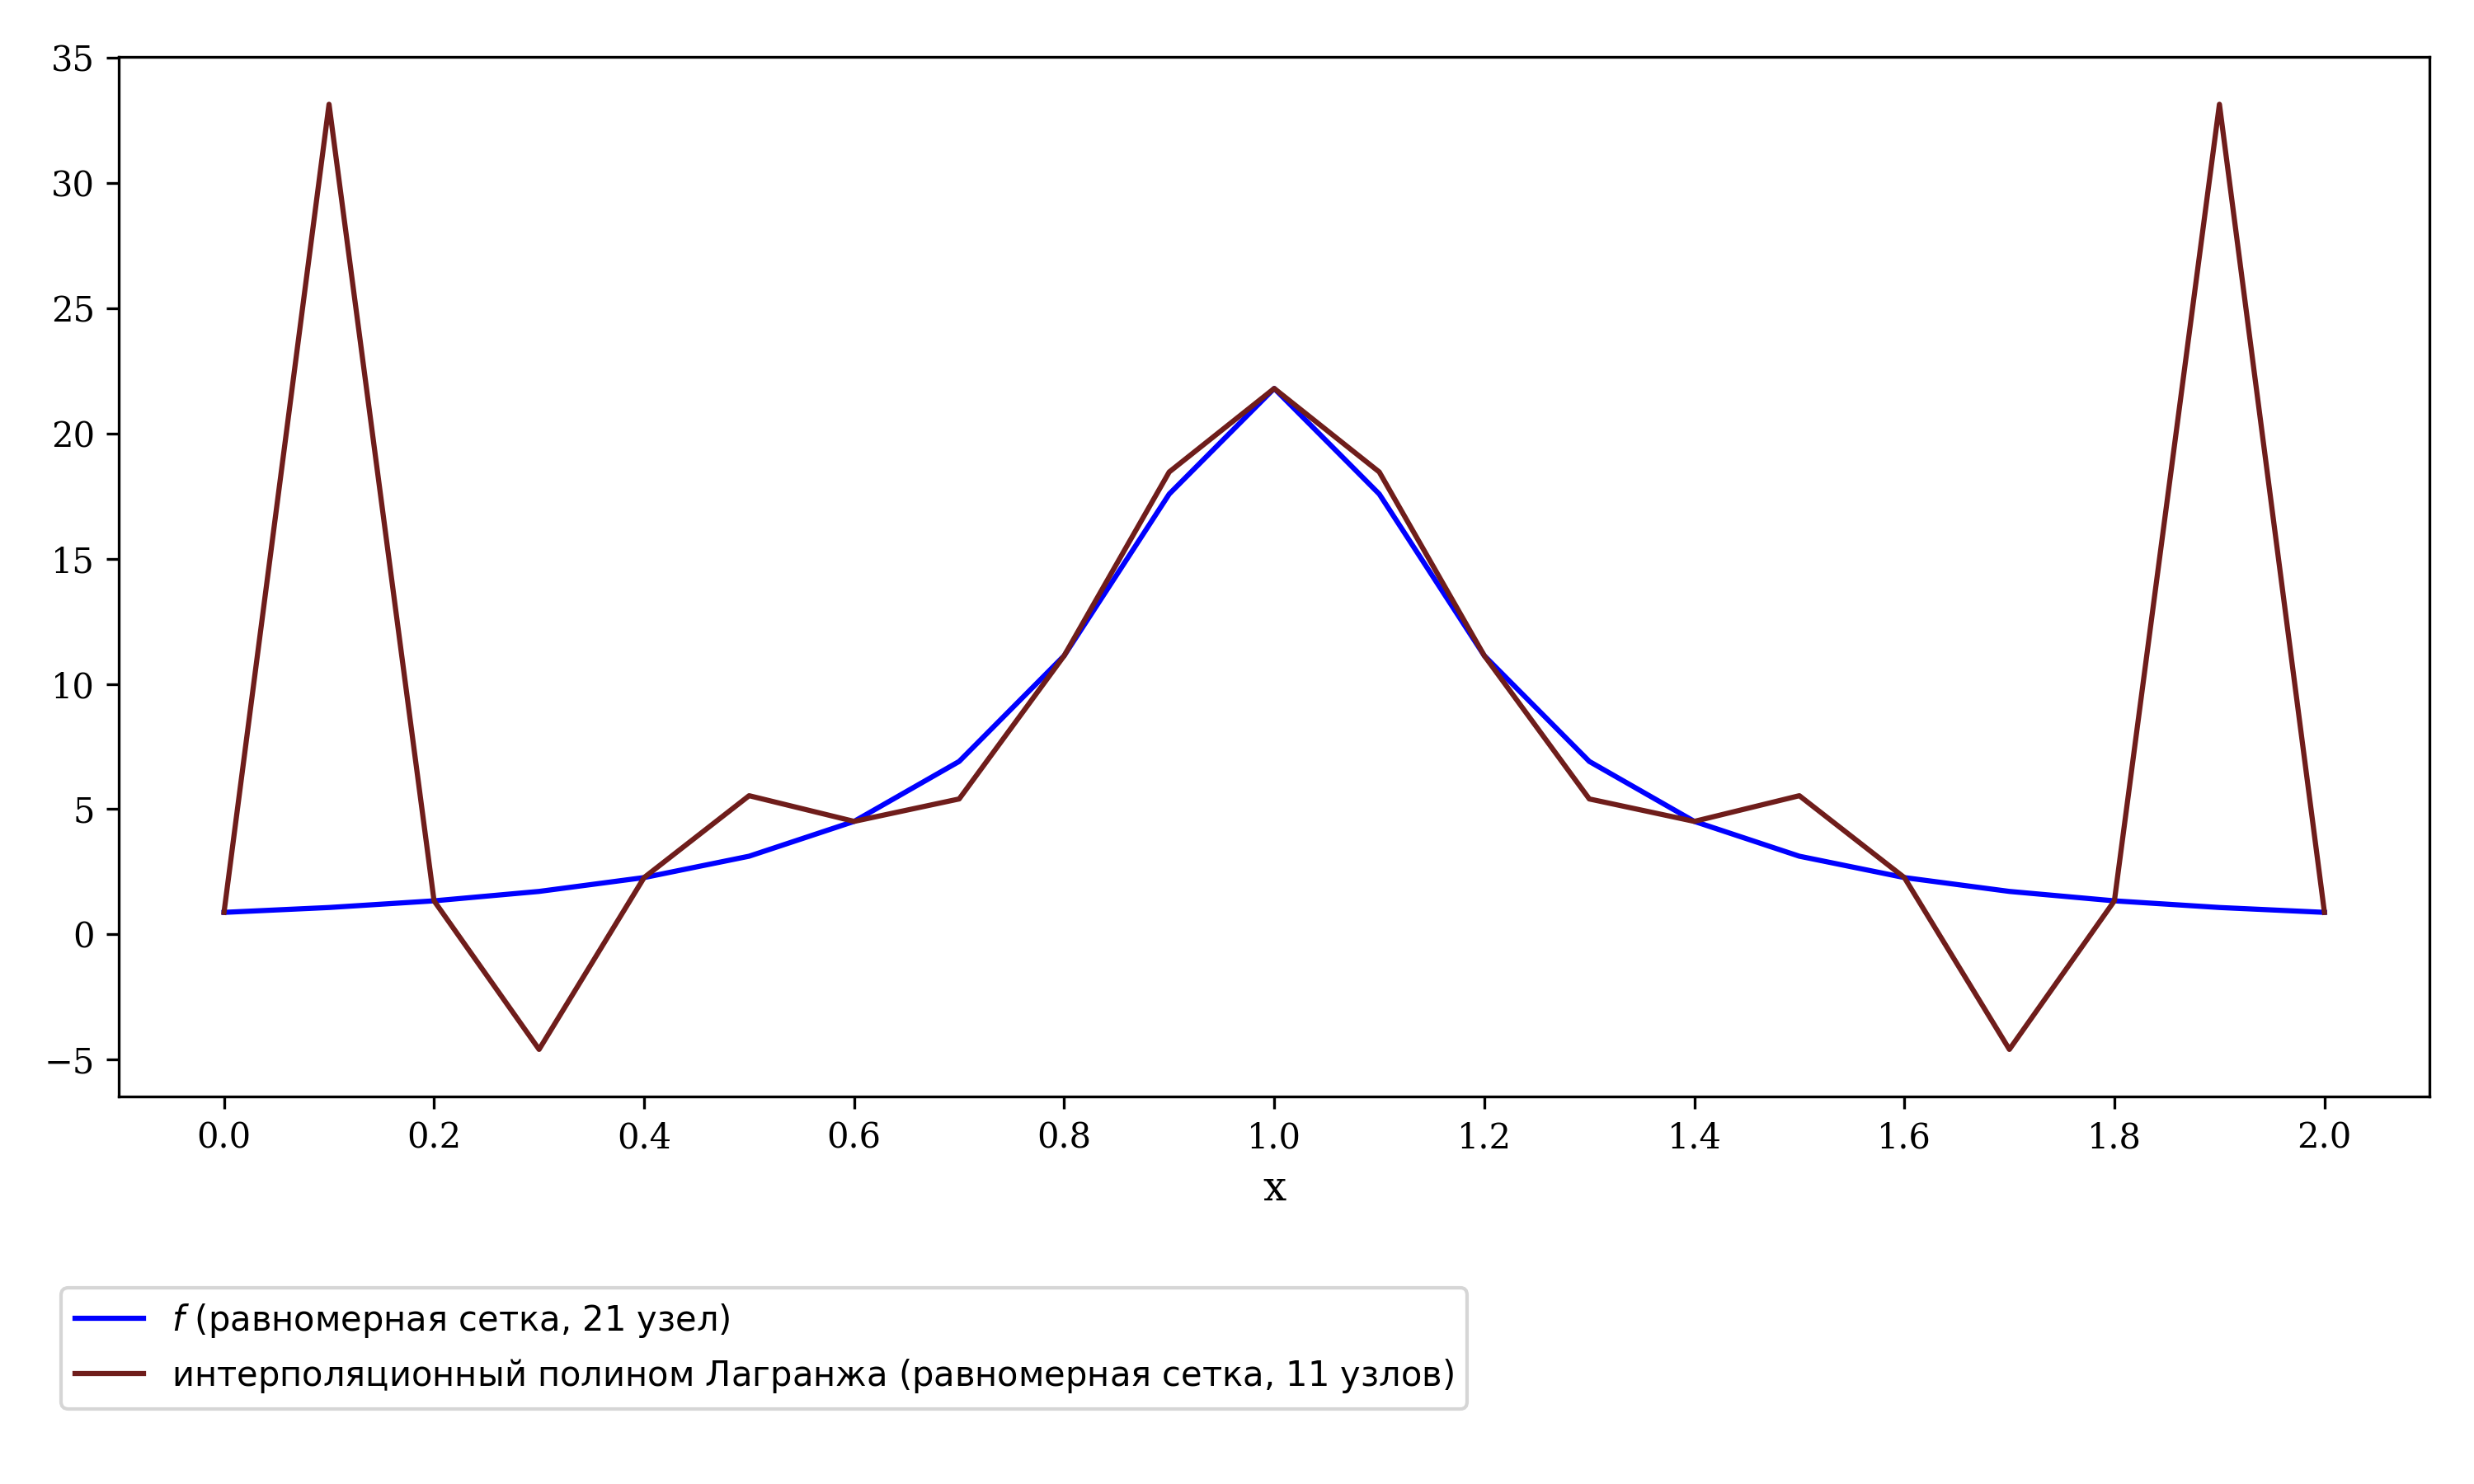
\includegraphics[width=1\textwidth]{uniformXref21}
\end{center}

\newpage

Также представим совмещенные графики функции $f$, и 
вычисленного (с 11-ю равномерными узлами) интерполяционного полинома Лагранжа, 
используя равномерную сетку с 1000 узлами.

\begin{center}
  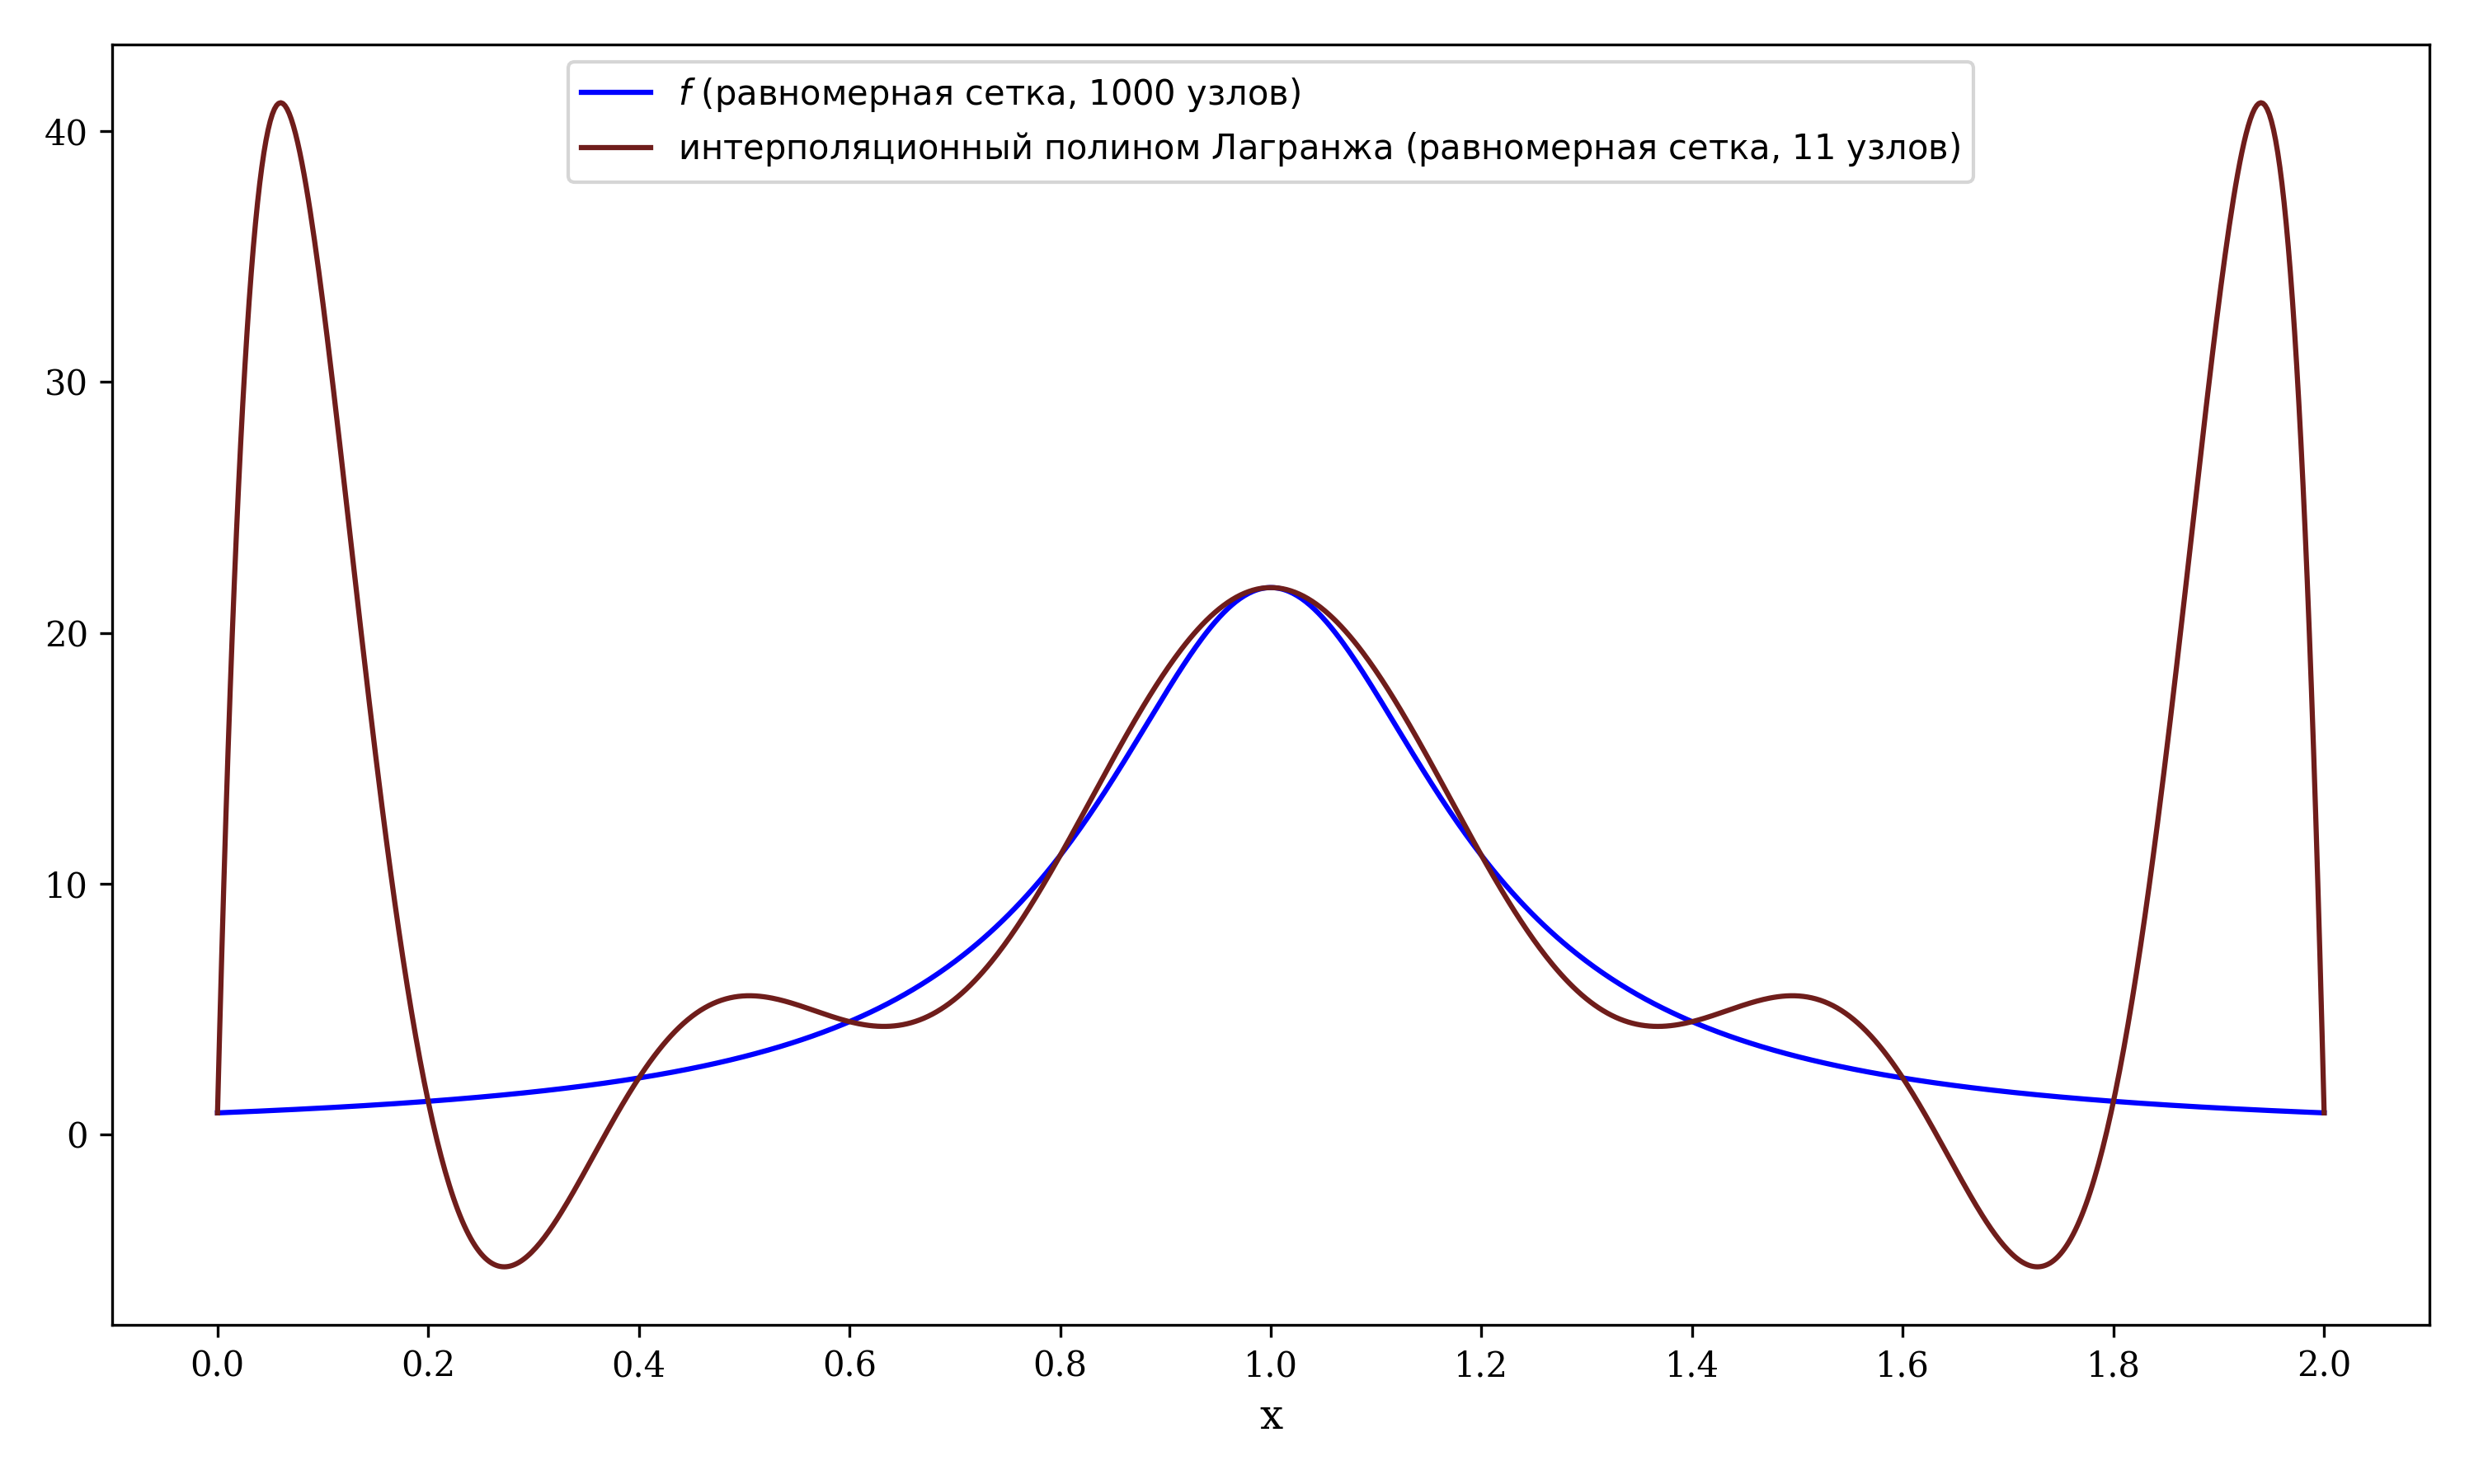
\includegraphics[width=1\textwidth]{uniformXref1000}
\end{center}

Как видно из графиков, на концах отрезков присутствует сильный 
эффект нежелательных осцилляций (феномен Рунге).

\subsection*{Часть 2}\vspace{-20pt}\rule{\linewidth}{0.1mm}

Используя чебышевскую сетку с 11-ю узлами, вычислить интерполяционный полином
Лагранжа.

\paragraph*{Чебышевская сетка}\vspace{-20pt}\rule{\linewidth}{0.1mm}

Для натурального числа n узлы Чебышёва на отрезке [-1, 1] задаются формулой 
\begin{equation*}
  x_k = \cos(\cfrac{2k - 1}{2n} \pi), \quad k=1,...,n.
\end{equation*}

Это корни многочлена Чебышёва первого рода степени n. 
Для получения узлов на произвольном отрезке [a, b] можно применить аффинное 
преобразование отрезков: 
\begin{equation*}
  x_k = \cfrac{1}{2} (a+b) + \cfrac{1}{2} (b-a) \cos(\cfrac{2k-1}{2n}\pi), \quad k=1,...,n.
\end{equation*}

Также вычислим значения функции $f(\tau)$ в узлах:
\begin{equation*}
  y_i = f(x_i), \qquad i=0,1,2,...,10,
\end{equation*}

Итого получим следующие точки:
\begin{multicols}{3}
  \begin{enumerate}[itemsep=5pt]
    \item (x: 0.01, y: 0.89)
    \item (x: 0.09, y: 1.046)
    \item (x: 0.244, y: 1.483)
    \item (x: 0.459, y: 2.722)
    \item (x: 0.718, y: 7.509)
    \item (x: 1.0, y: 21.8)
    \item (x: 1.282, y: 7.509)
    \item (x: 1.541, y: 2.722)
    \item (x: 1.756, y: 1.483)
    \item (x: 1.91, y: 1.046)
    \item (x: 1.99, y: 0.89)    
  \end{enumerate} 
\end{multicols}

\vspace{10pt}

\begin{center}
  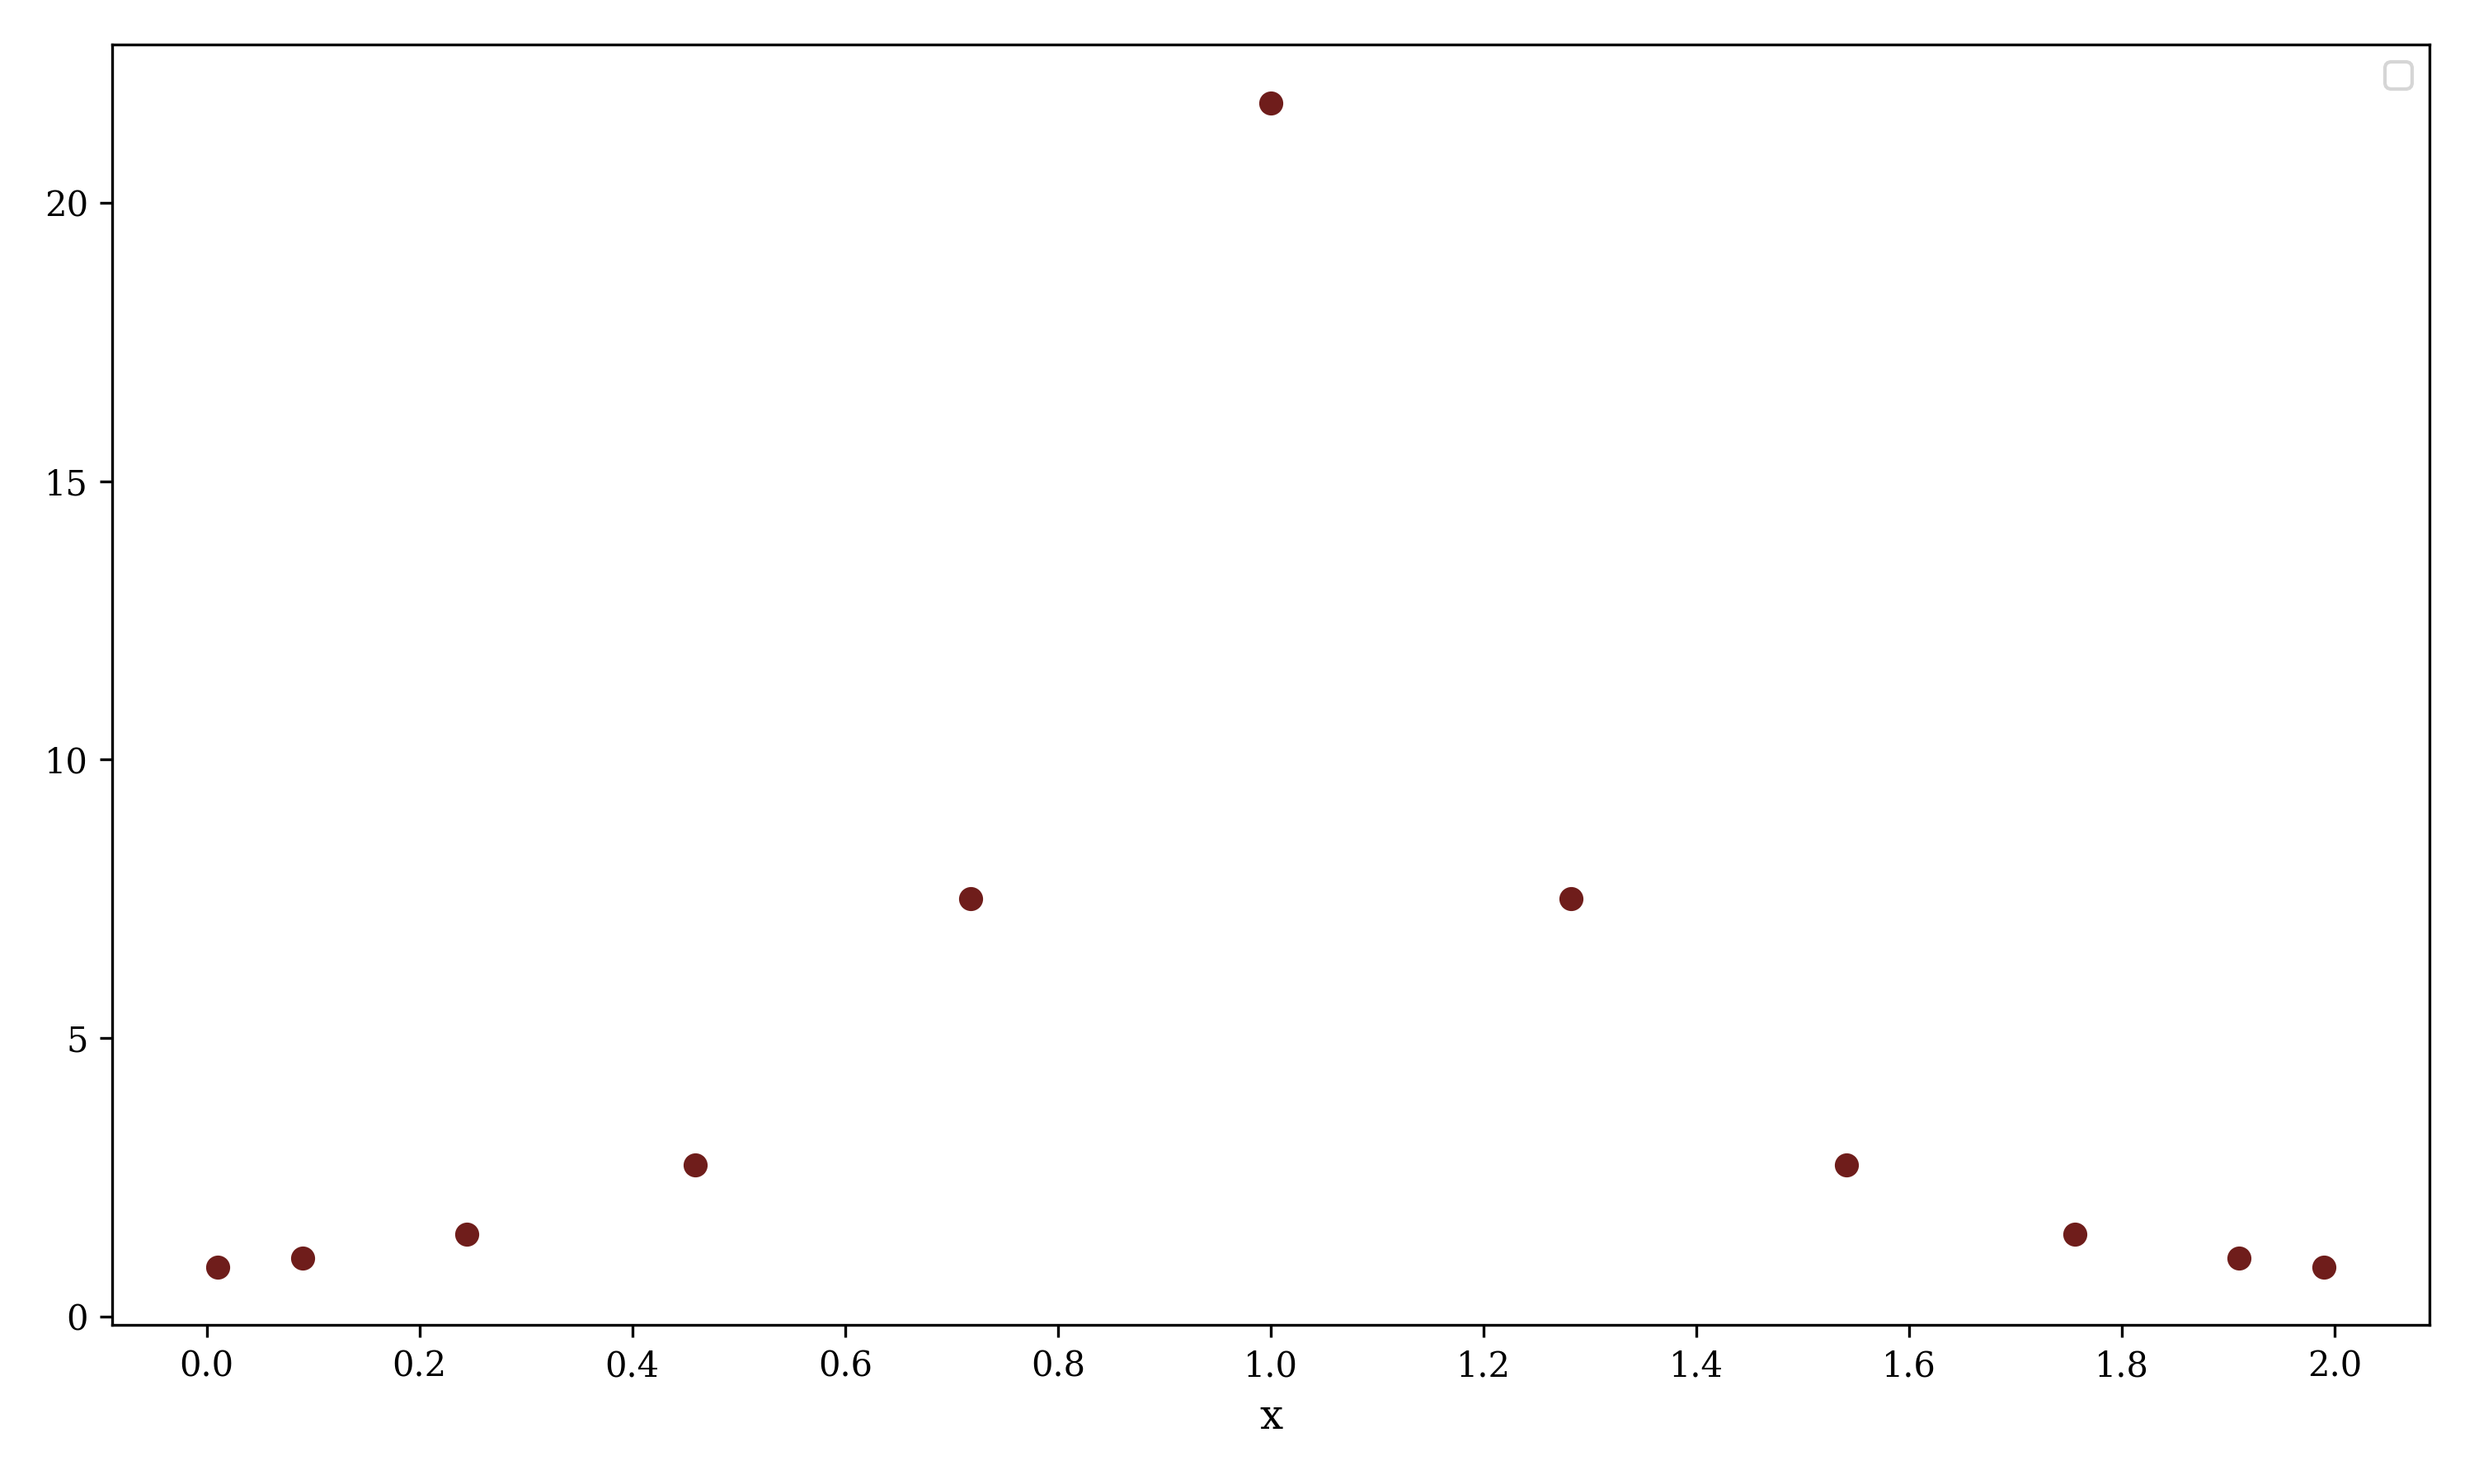
\includegraphics[width=1\textwidth]{scatter2}
\end{center}

\newpage

\paragraph*{Интерполяционный многочлен Лагранжа (с использованием чебышевской сетки с 11-ю узлами)}\vspace{-20pt}\rule{\linewidth}{0.1mm}

Представим совмещенные графики функции $f$, используя равномерную сетку с 21 узлом и 
вычисленного (с 11-ю чебышевскими узлами) интерполяционного полинома Лагранжа.

\begin{center}
  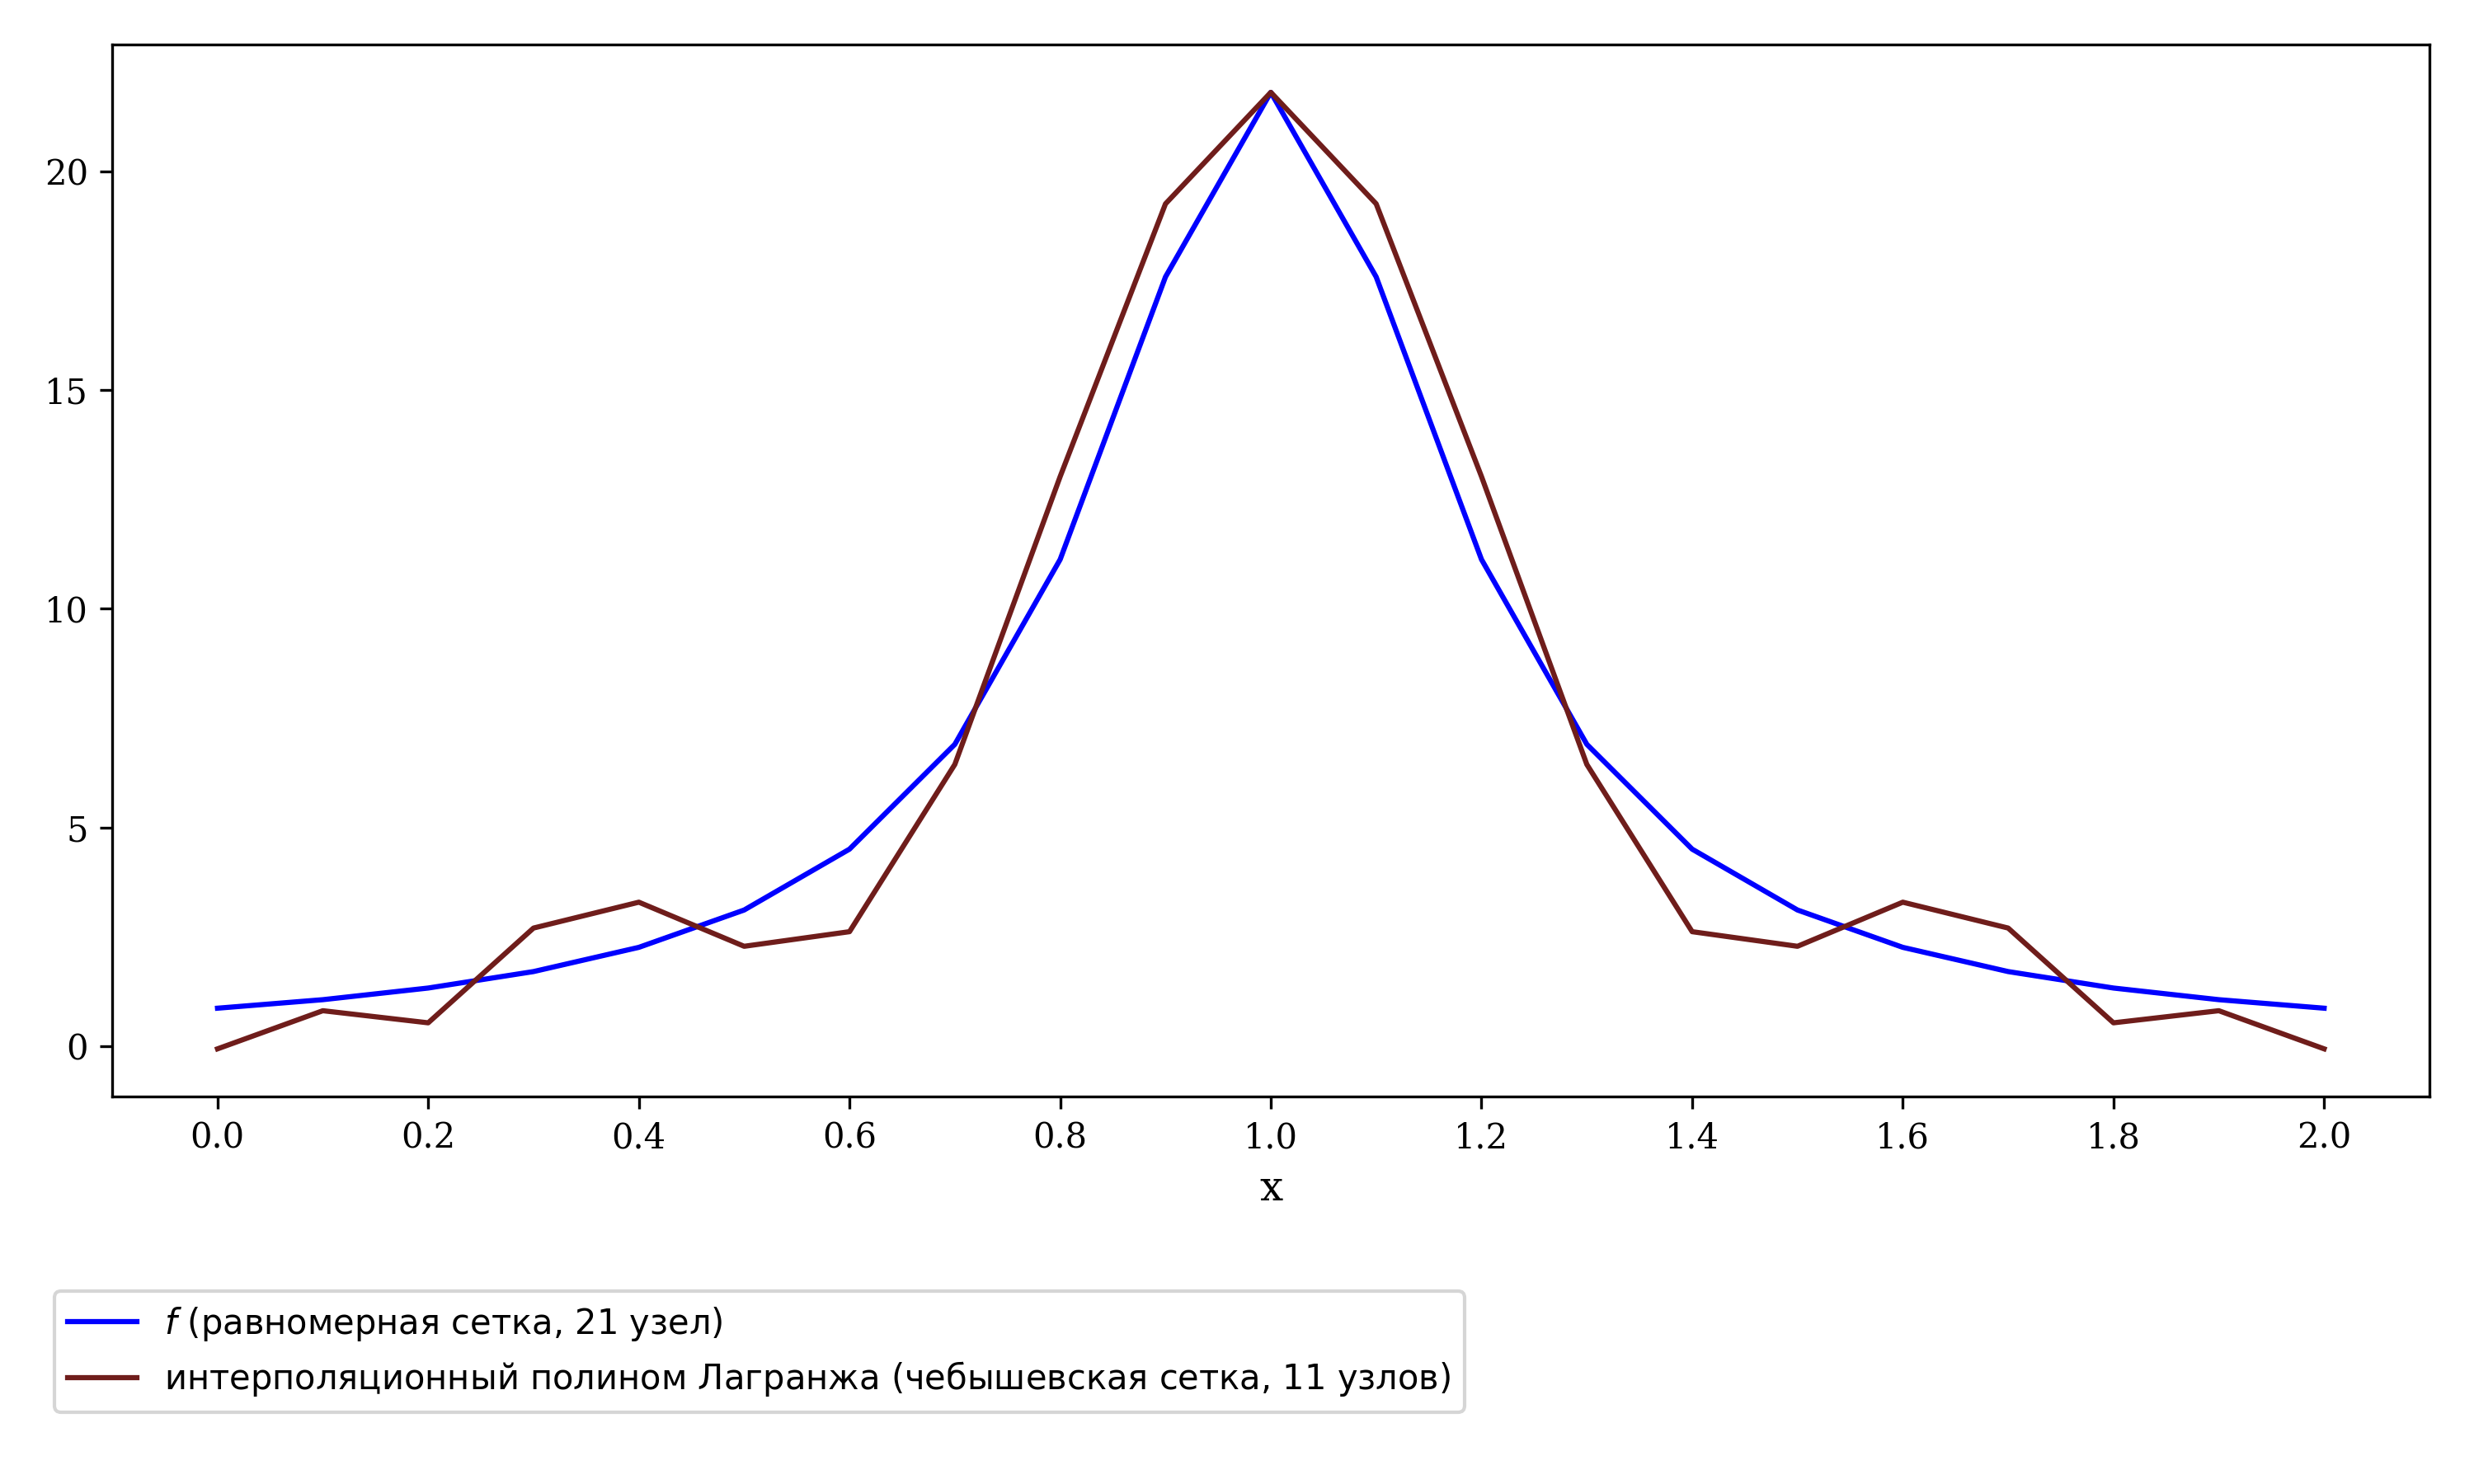
\includegraphics[width=1\textwidth]{chebushevXref21.png}
\end{center}

Также представим совмещенные графики функции $f$, и 
вычисленного (с 11-ю чебышевскими узлами) интерполяционного полинома Лагранжа, 
используя равномерную сетку с 1000 узлами.

\begin{center}
  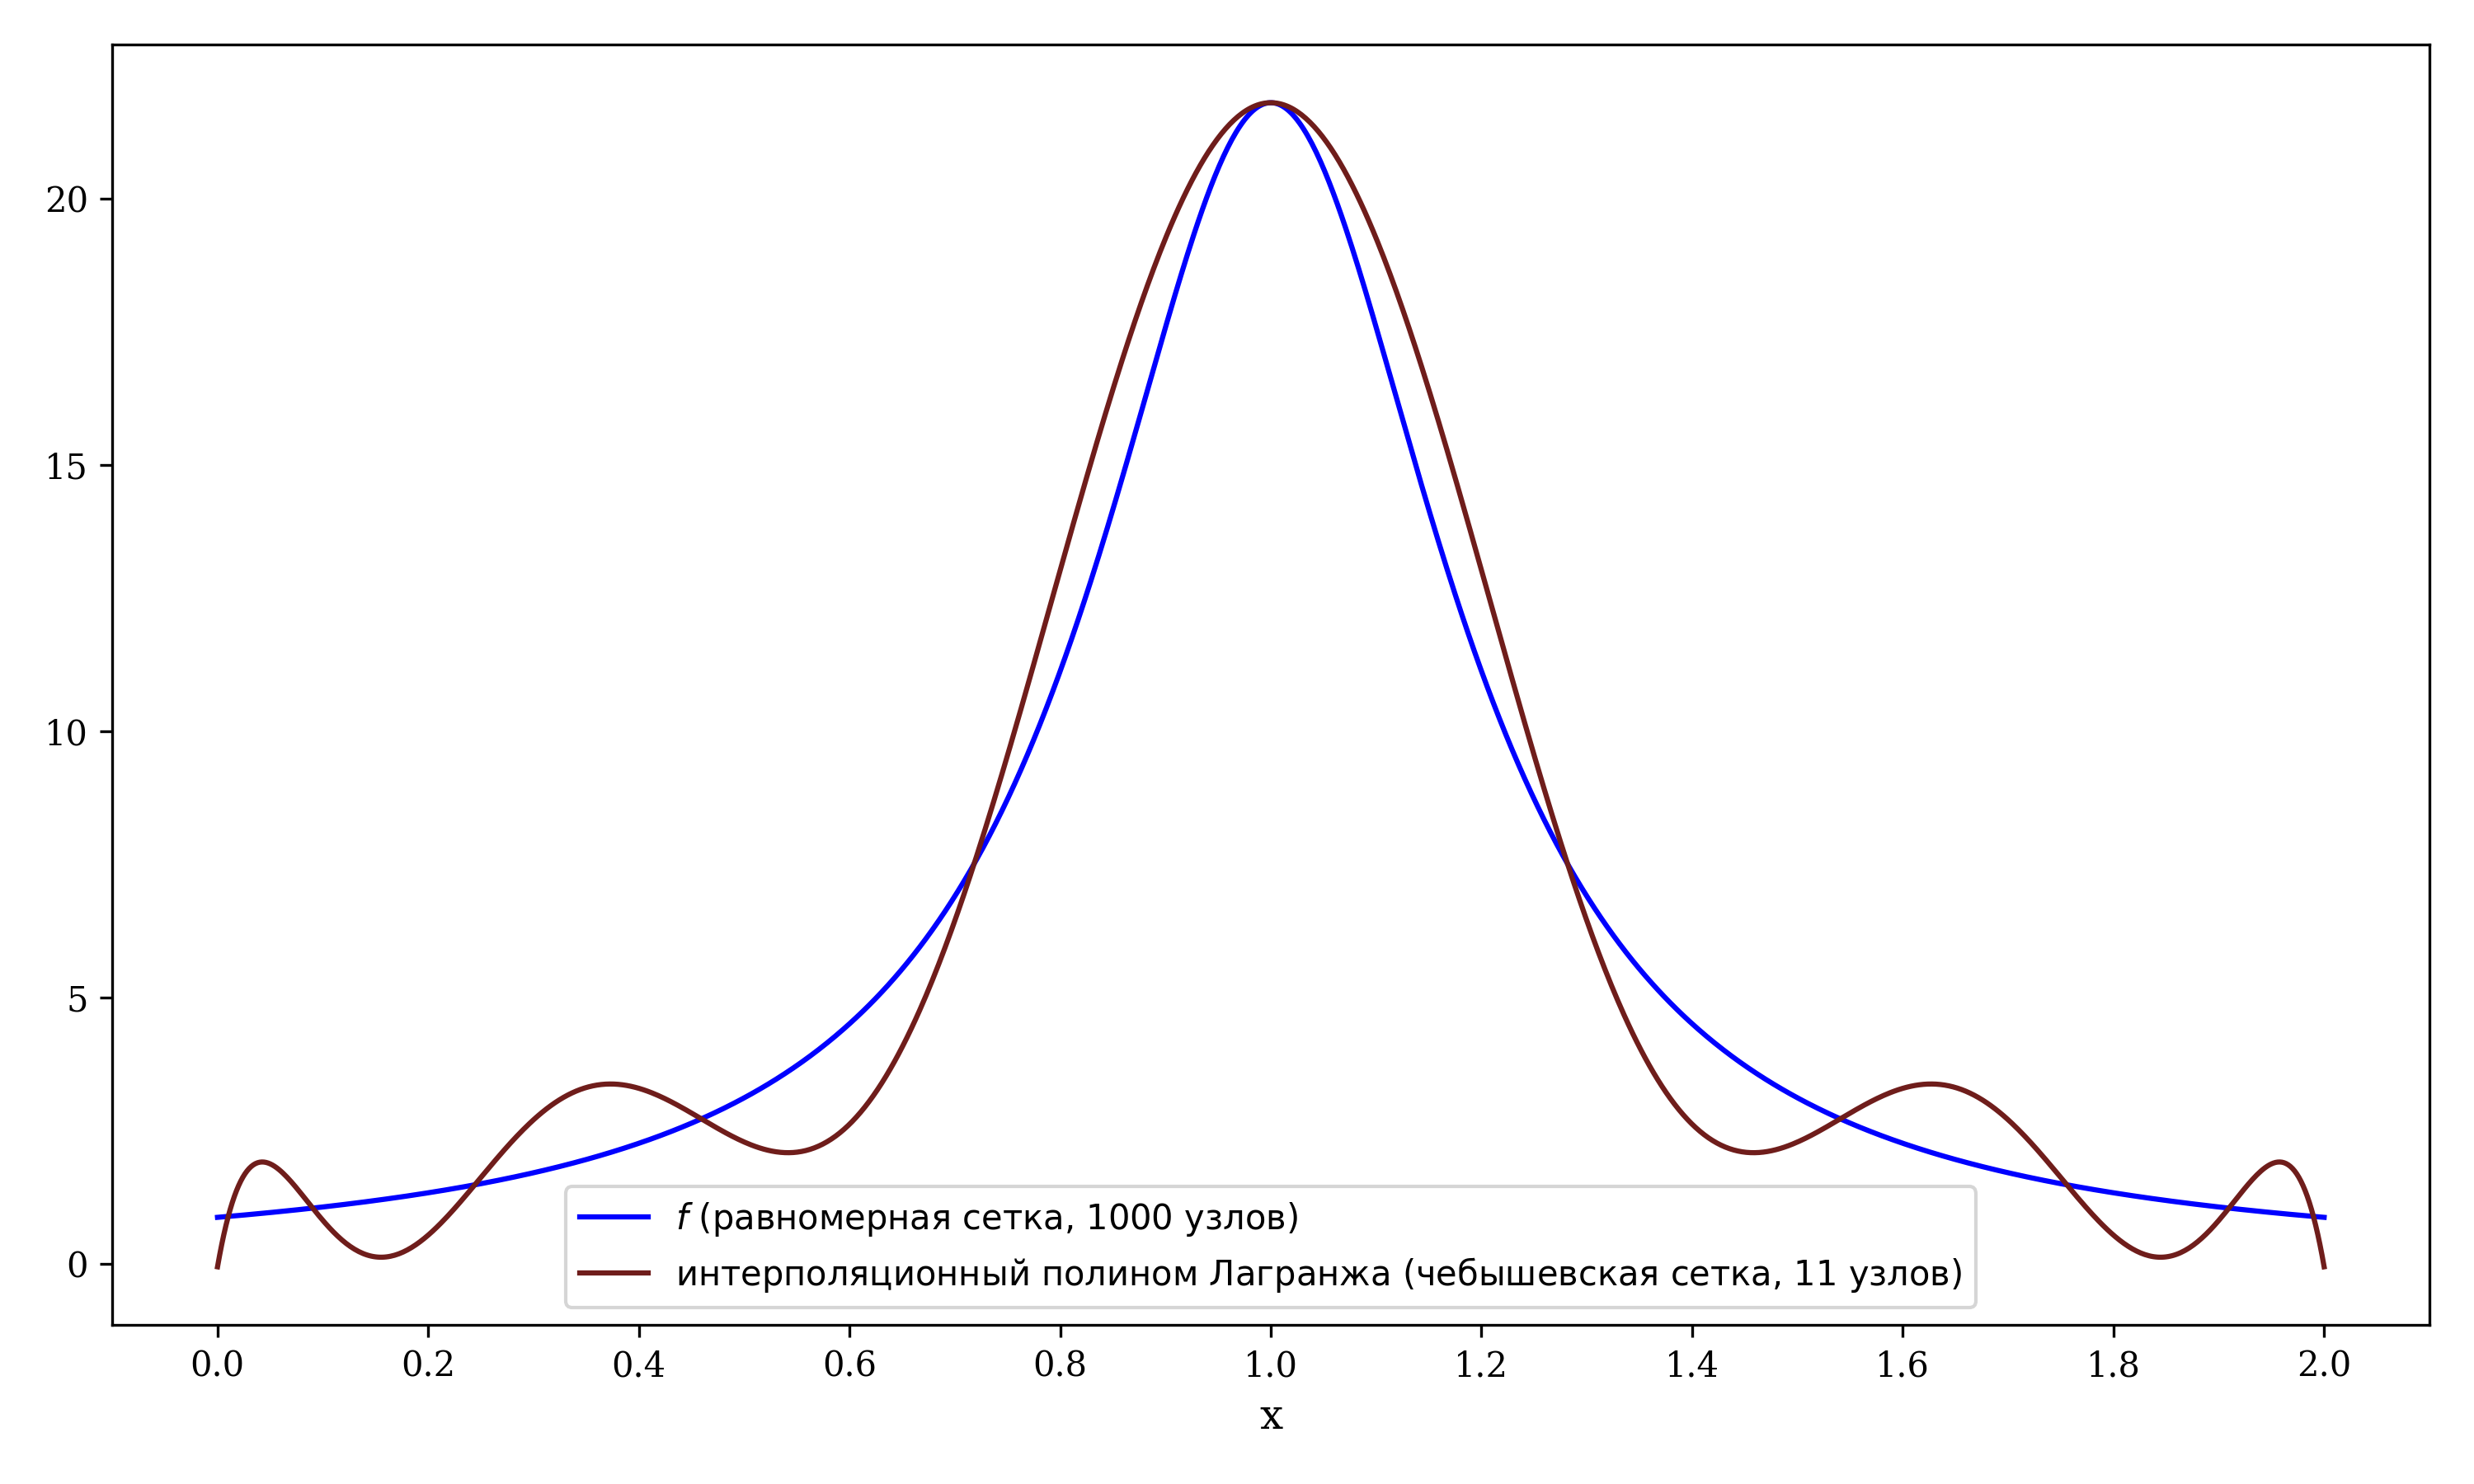
\includegraphics[width=1\textwidth]{chebushevXref1000}
\end{center}

Благодаря тому, что в этот раз была использована Чебышевская сетка, нам удалось 
снизить влияние феномена Рунге.

\subsection*{Часть 3}\vspace{-20pt}\rule{\linewidth}{0.1mm}

Дополнительно изобразим совмещенные графики полученных интерполяционных полиномов Лагранжа 
с 11-ю равномерными и с 11-ю чебышевскими узлами, используя равномерную
сетку с 21 узлом.

\begin{center}
  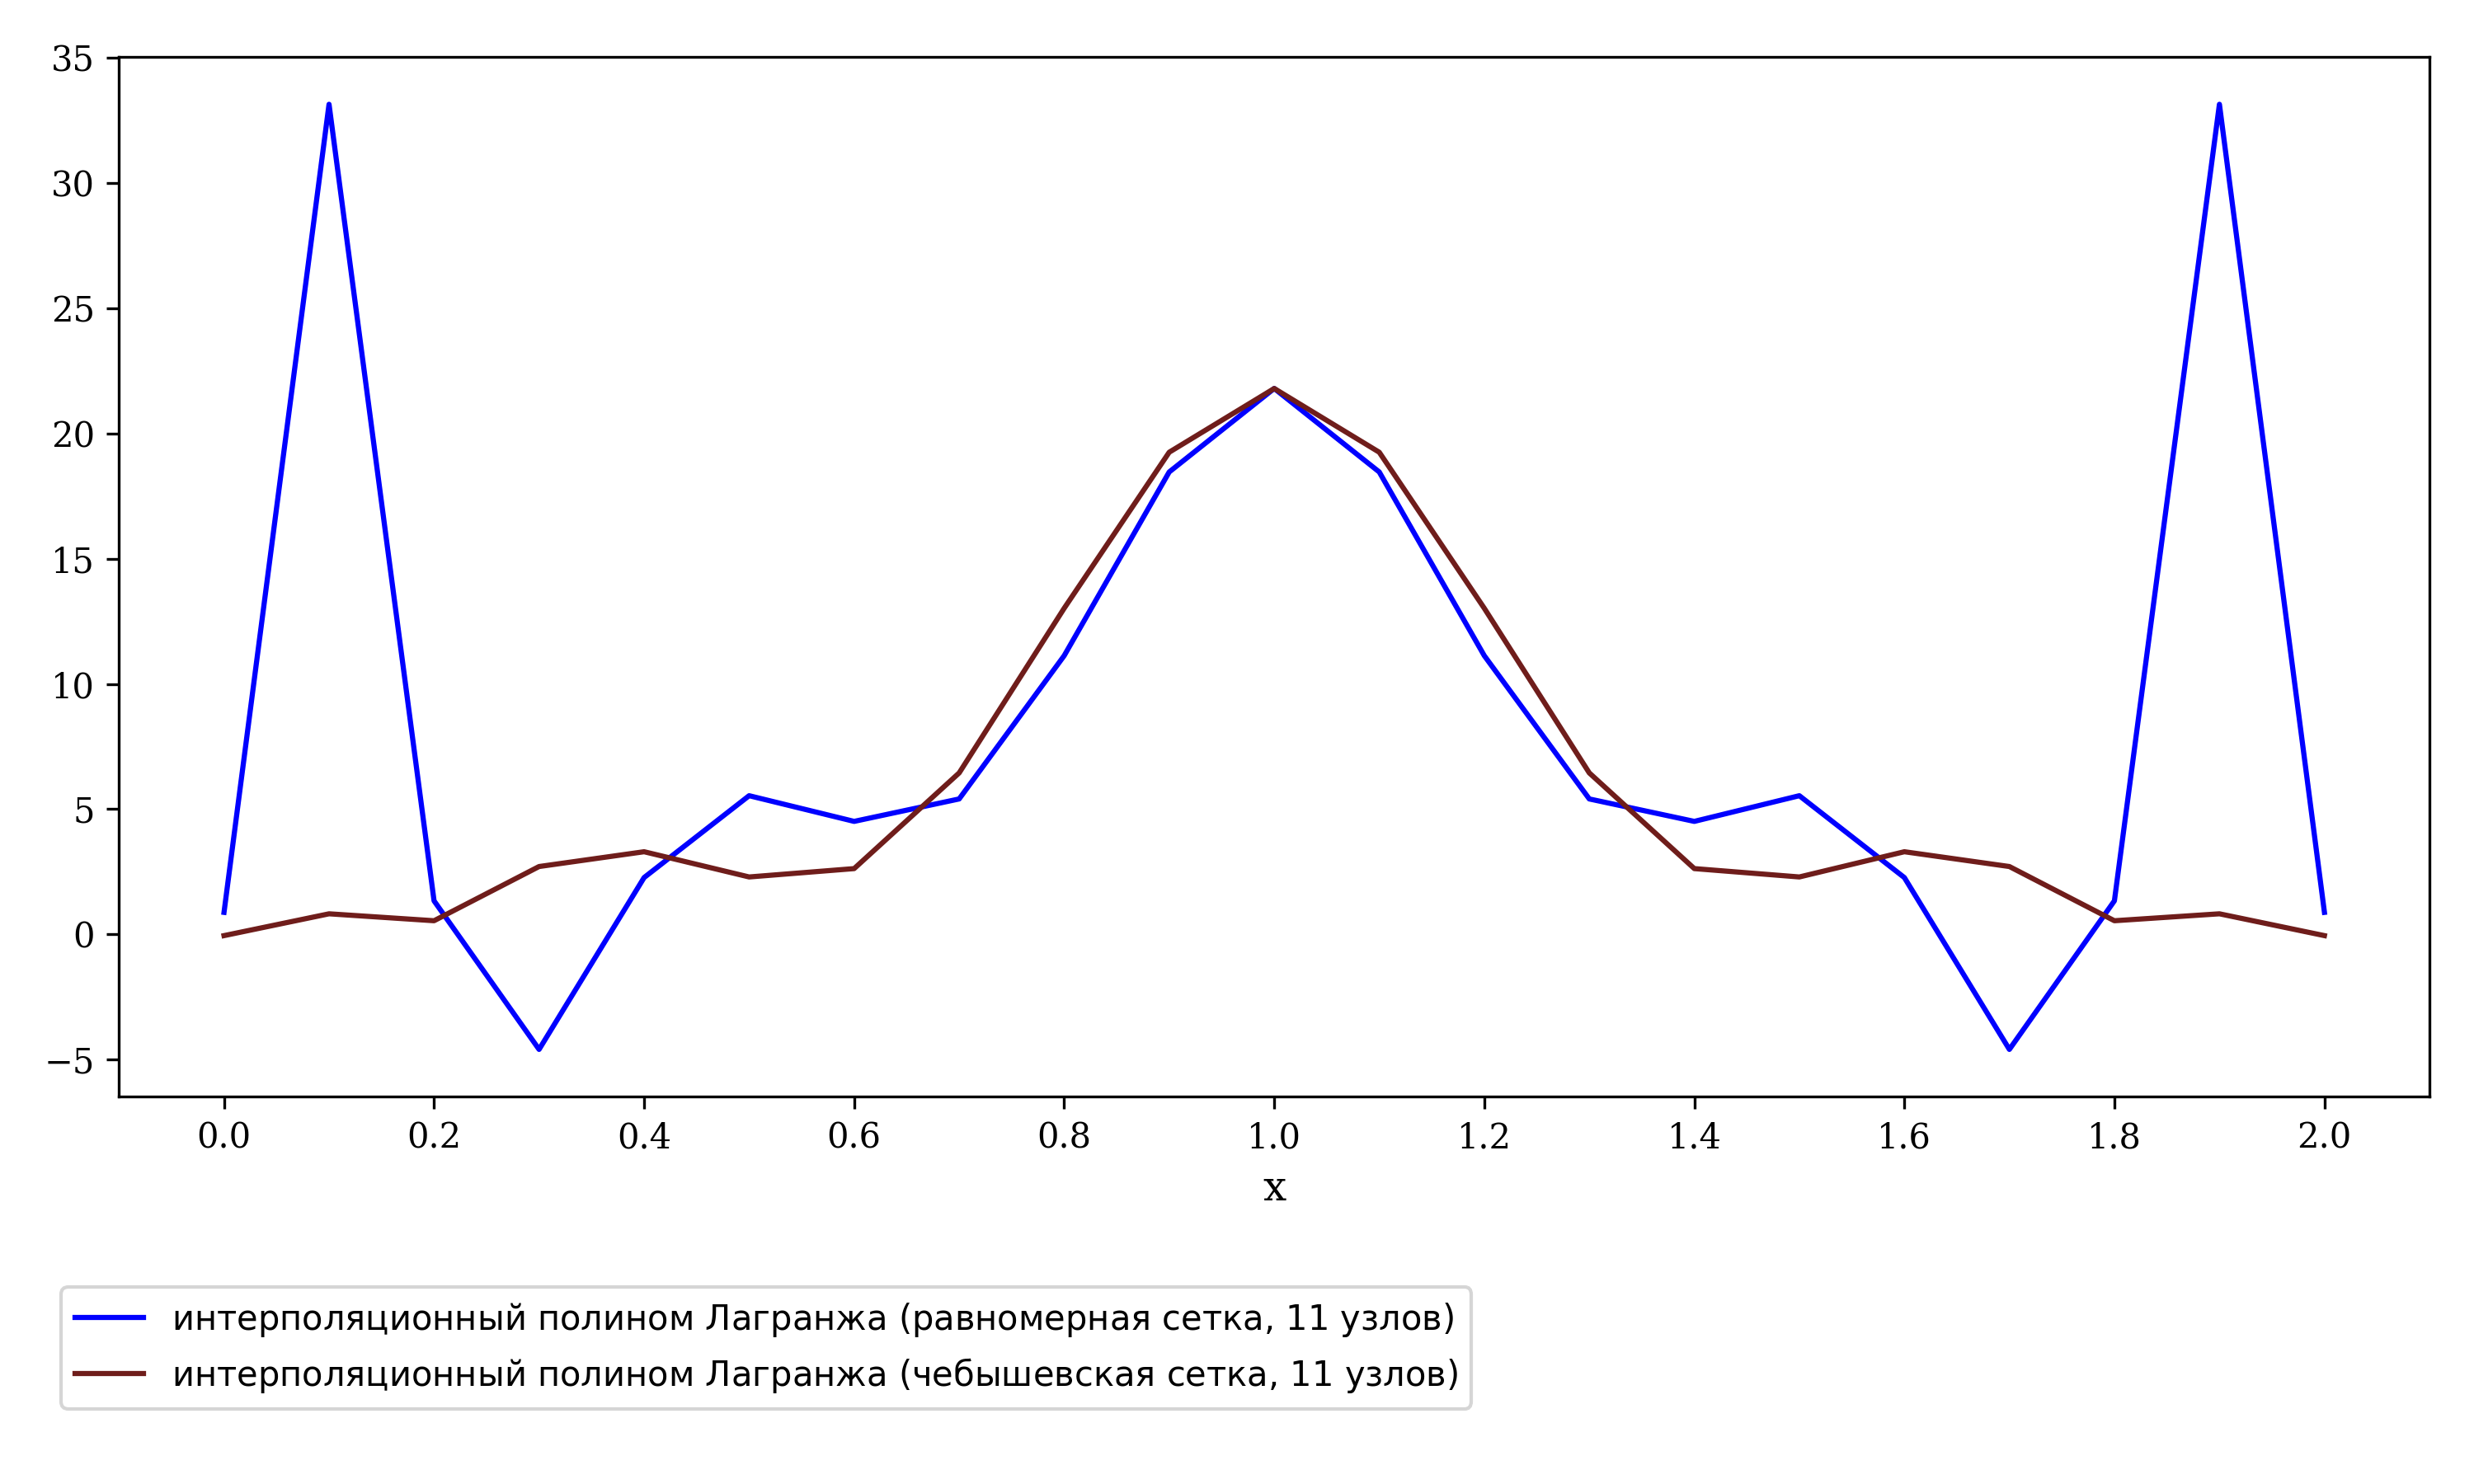
\includegraphics[width=1\textwidth]{uniformXchebushev21}
\end{center}

и с 1000 узлами.

\begin{center}
  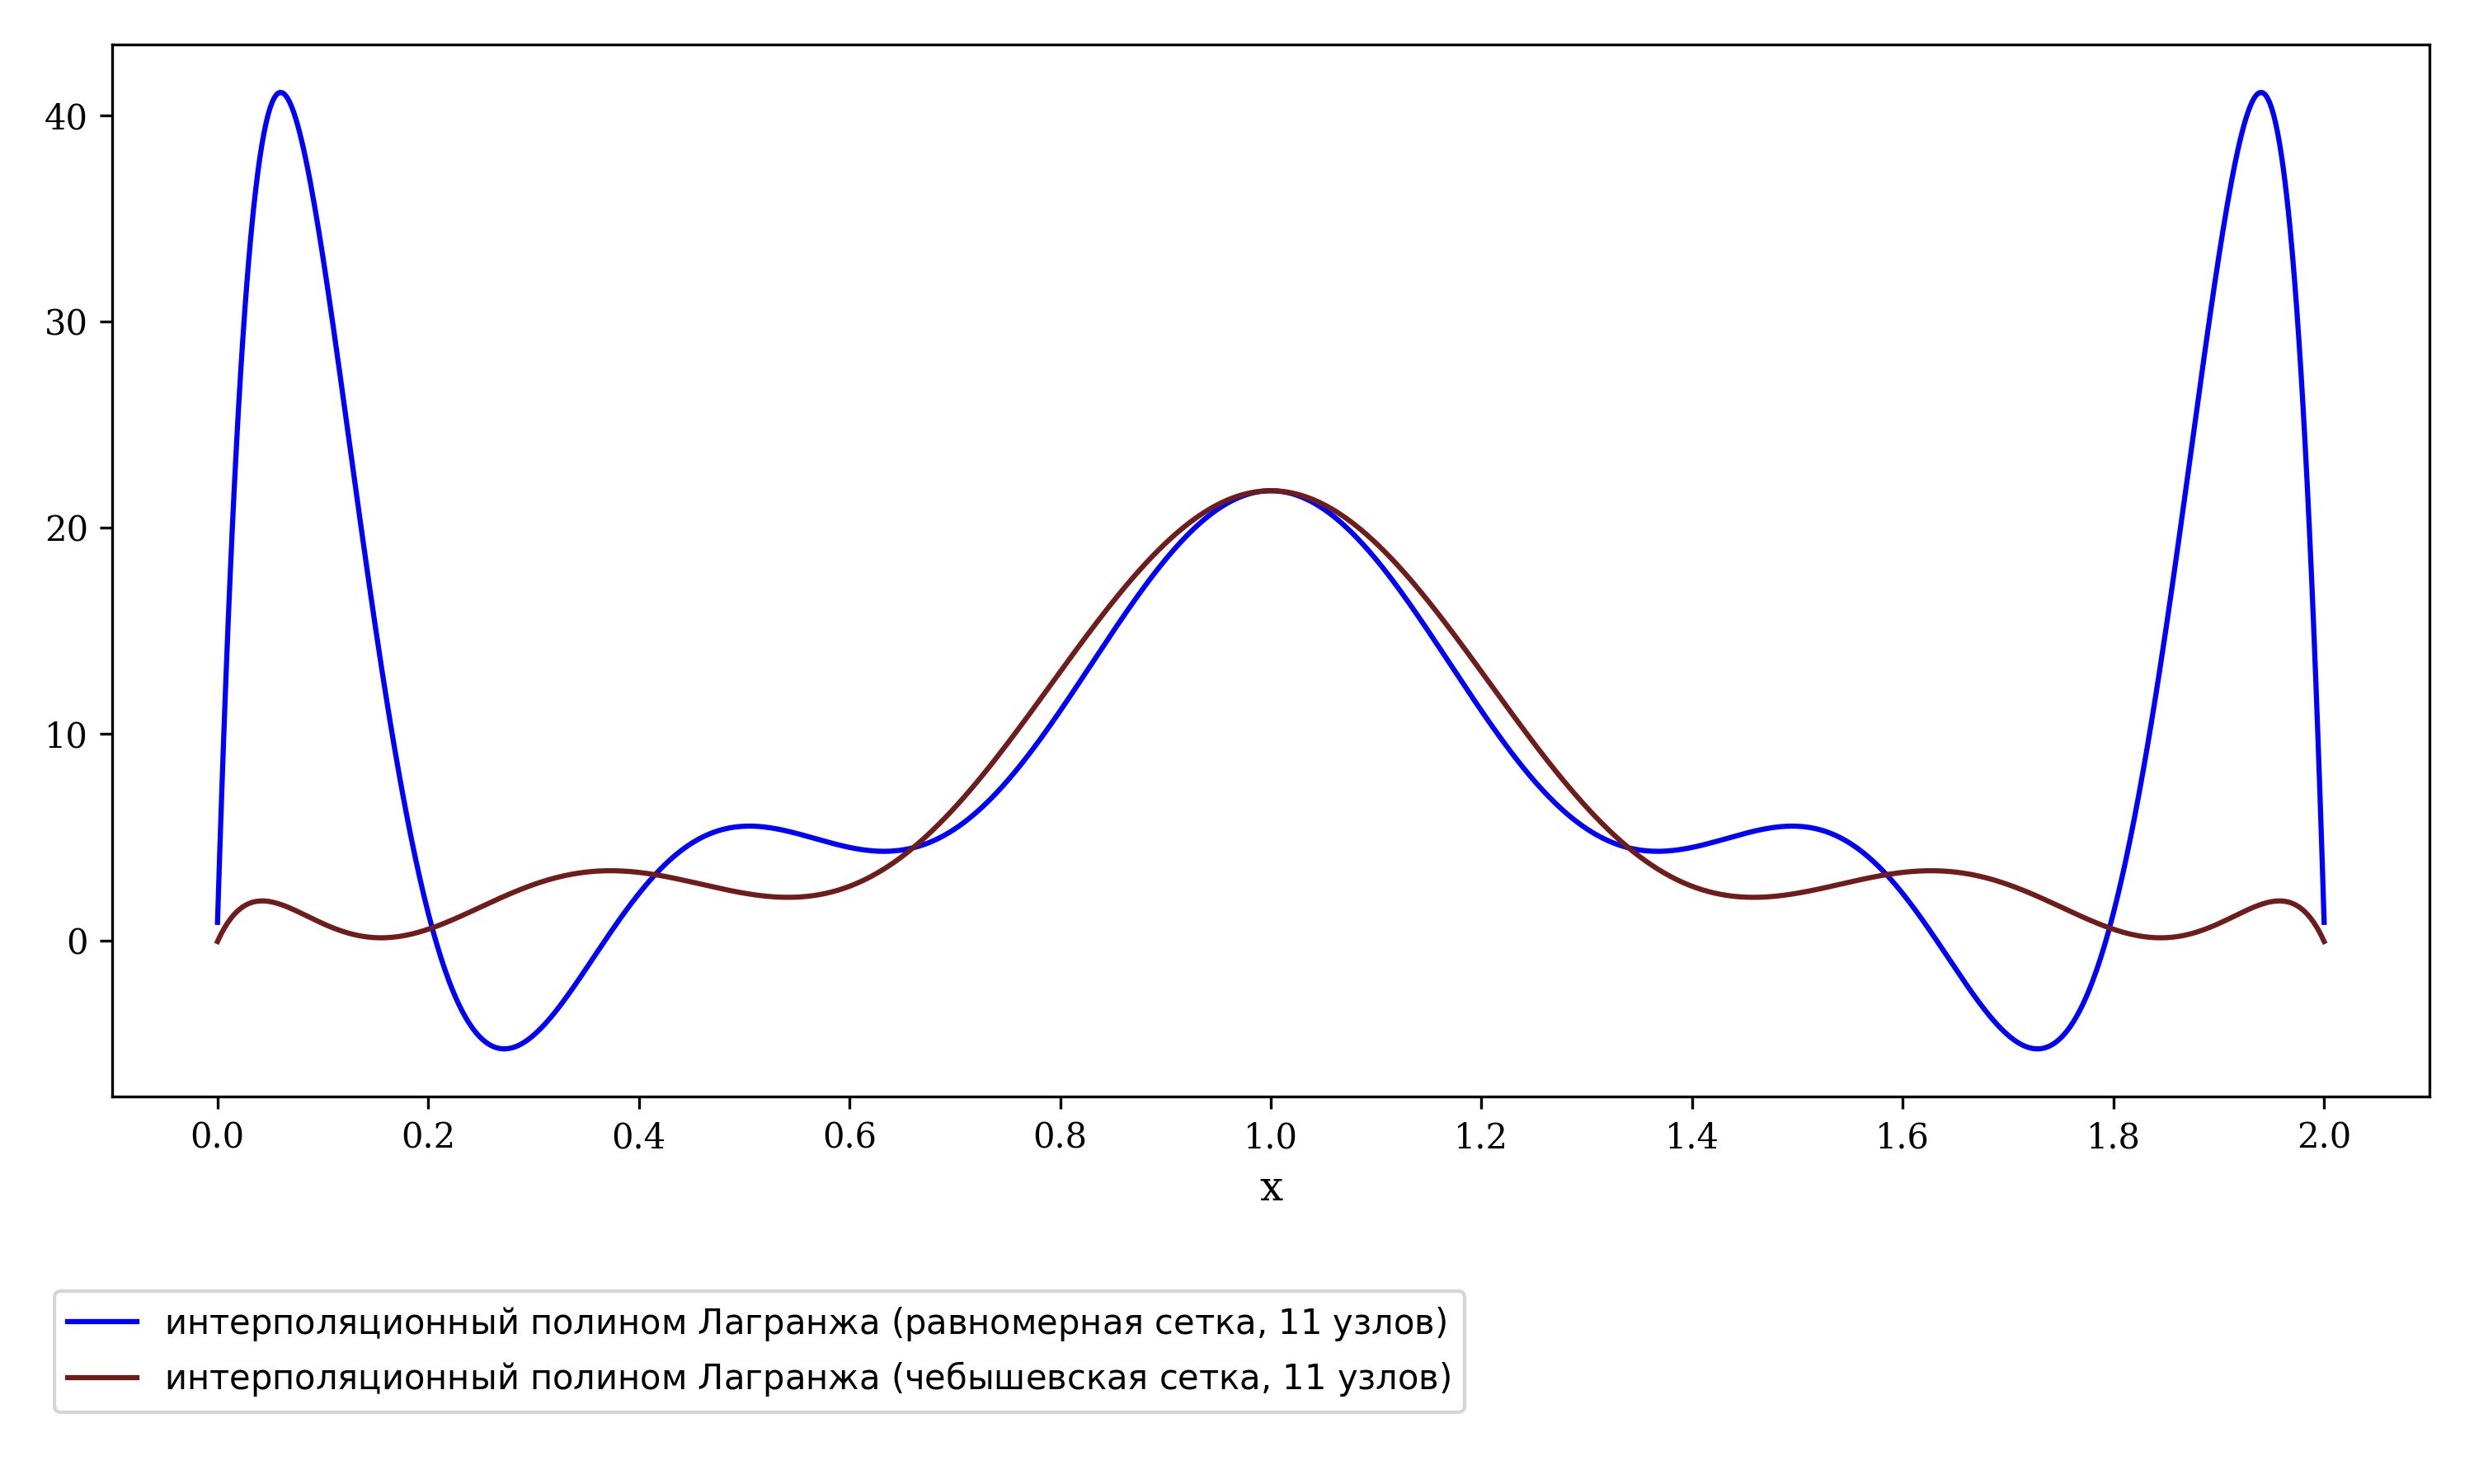
\includegraphics[width=1\textwidth]{uniformXchebushev1000}
\end{center}

А также добавим эталонный график.

\begin{center}
  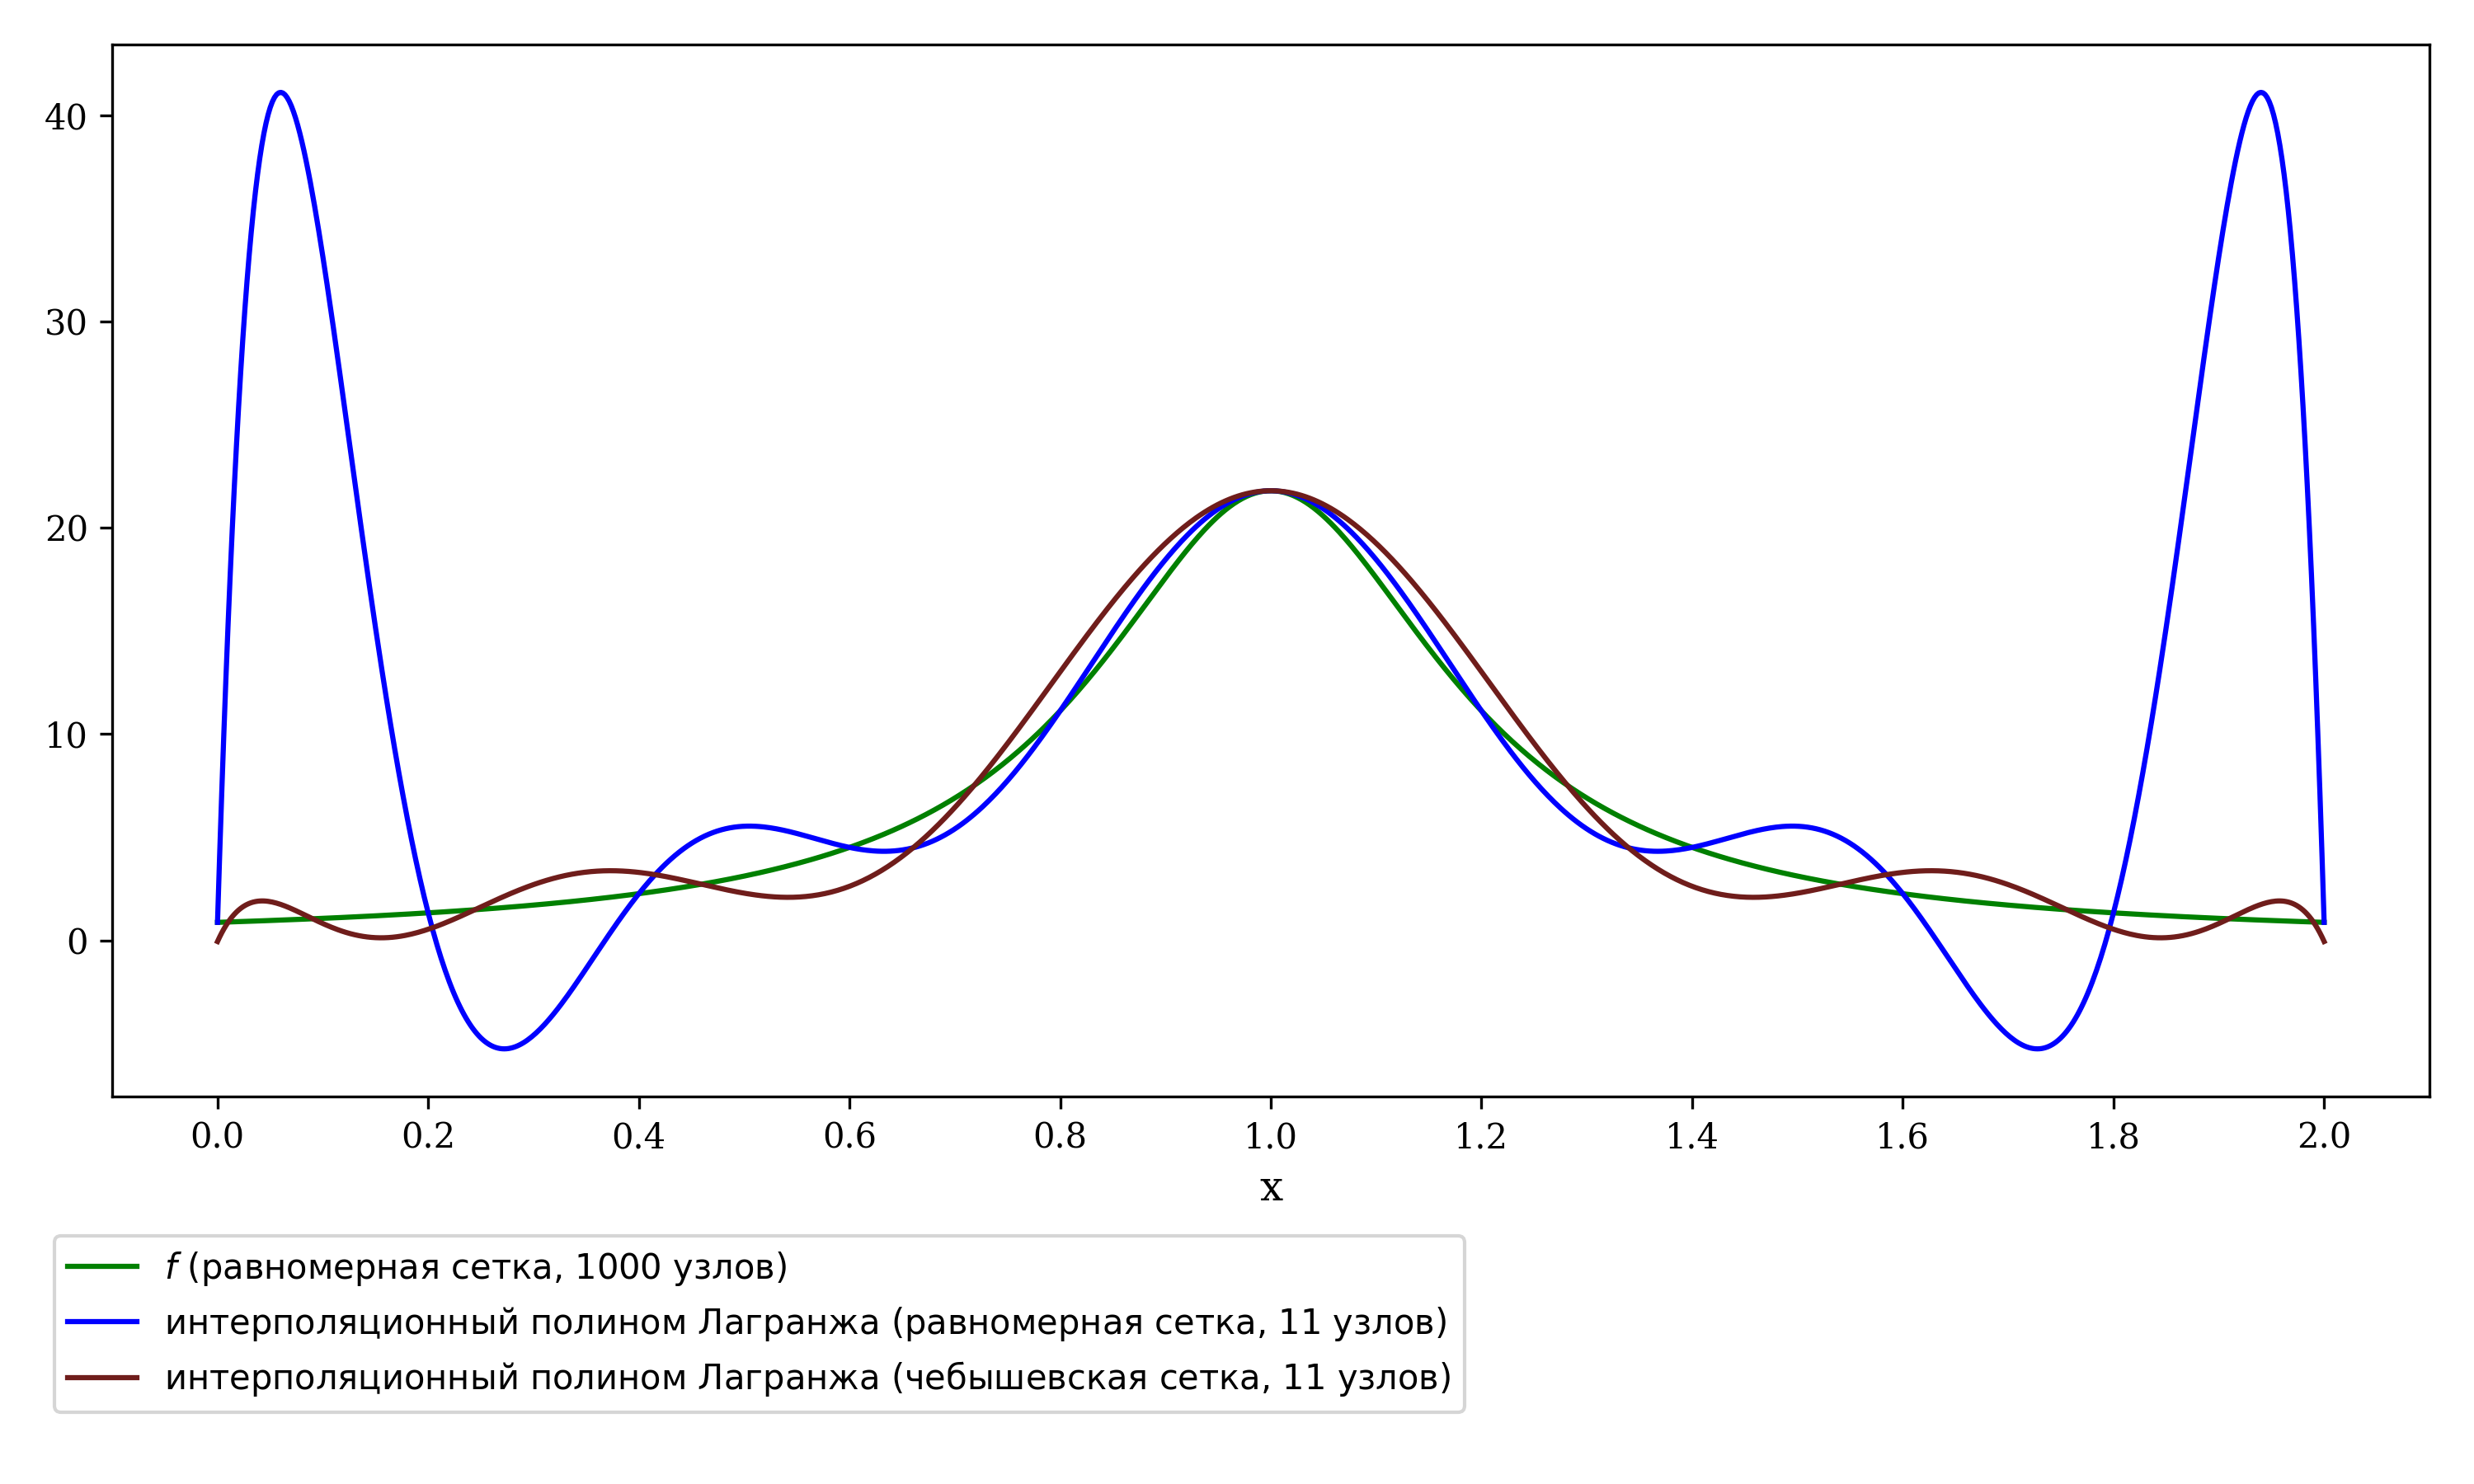
\includegraphics[width=1\textwidth]{uniformXrefXchebushev1000}
\end{center}

\section*{Вывод}\vspace{-20pt}\rule{\linewidth}{0.1mm}

В ходе проделанного домашнего задания были вычислены интерполяционные полиномы Лагранжа, 
с использованием равномерной и Чебышевской сетки с 11-ю узлами. Исходя из результов работы, 
можно сделать вывод, что при втором способе вычисления, 
значительно снижается эффект нежелательных колебаний.

\end{document}
